\section{基于随机森林相似性学习的单细胞聚类方法}
\label{sec:rafclust}

\subsection{引言}

前面两章在基于~DNA~微阵列数据上的分别介绍了两种基因调控网络的构建方法,
一个是注重无向的网络结构推断, 另一个则是有向的整体网络推断。
当使用的数据转向了单细胞~RNA-seq~数据集的时候, 由于单细胞数据本身独有的特点, 基因调控网络的推断过程变得复杂起来。
基因调控与细胞类型密切相关~\cite{Hocker2020.09.11.291724,kang2020learning},
细胞聚类也是单细胞~RNA-seq~数据分析的热门和重要的问题, 
因此构建基因调控网络的一个不可或缺的前置任务是在单细胞数据集上对细胞的异质性进行聚类分析。

本章中,我们提出了一种高效准确的单细胞聚类方法~RafClust。
针对当前单细胞~RNA-seq~数据集上细胞聚类不够准确鲁棒的问题,
我们使用多种相关性度量方法来刻画细胞的特征, 
然后使用随机森林回归模型进一步学习细胞与细胞之间的相似性矩阵,
基于相似性矩阵后采用层次聚类来决定细胞的最终类别。
实验结果表明, 在十个单细胞数据集上,~RafClust~在~ARI~上表现优于其它六种方法。

\subsection{相关工作}

单细胞~RNA-seq~(scRNA-seq)~技术提供了单细胞水平的转录组测量。
使不同组织中细胞类型的鉴定和表示成为可能。
相比之下,传统的批量~RNA~测序的表达值是数千或数百万细胞的平均值,因此存在局限性。
单细胞~RNA-seq~技术的出现提供了一个从细胞水平研究生物机制的前所未有的视角,
能够从基因、调控、表达等多方面解释细胞变化的原因,
使得研究人员更严格地处理一些生物问题,比如组织的细胞组成、转录组的异质性,
以及细胞在发育过程中或在疾病和癌症中类型是如何的变化~\cite{kumar2017understanding,patel2014single}。

基于单细胞~RNA-seq~的细胞异质性研究主要是根据每个细胞的基因表达量来计算细胞之间的相似性,
结合聚类方法来确定细胞的类别。
由于单细胞~RNA-seq~对于每个细胞测得读数有限,细胞在测序过程中也会发生粘连,导致每个细胞很多的基因表达量为~0,
这种现象被称之为单细胞的~dropout~\cite{vallejos2017normalizing}。
同时,单细胞~RNA-seq~测序中将基因作为特征,常见的人和老鼠两种物种都有~20000~多个基因,
这种高维特征也给单细胞~RNA-seq~数据上的聚类带来挑战~\cite{stegle2015computational}。
国内外研究者针对单细胞~RNA-seq~数据上的异质性研究已取得不少成果。
一类方法是最传统的聚类方法,比如使用~t-SNE~对数据进行降维然后使用~K-means~对数据进行聚类。
显然这种方法对噪声十分敏感。
Gr{\"u}n~等人~\cite{grun2016novo}~提出的~RaceID2~
使用~K-medoids~方法聚类,依据类内散布饱和临界值为依据确定分类个数。
另一类方法的研究思路是通过对原始数据进行插值处理~(imputation),减轻~scRNA-seq~数据中的~dropout~的影响。
典型的方法比如~Lin~等人提出的~CIDR~方法~\cite{lin2017cidr}。
CIDR~对~dropout~与基因表达值的关系进行了建模, 通过隐式插值处理后获取细胞与细胞之间的非相似性矩阵,
然后使用层次聚类获得最终的结果。
还有一类最流行的方法的研究思路是通过提高细胞与细胞之间的相似性计算的准确度和鲁棒性。
Kiselev~等人~\cite{kiselev2017sc3}~提出了一种共识聚类方法~SC3。
SC3~基于计算细胞与细胞间的~Pearson、Spearman~和欧氏距离三种不同相似性和主成分分析、拉普拉斯转换分别获得多个聚类结果,
然后通过计算这些聚类结果中两个细胞被聚为一类的数目来构建共识矩阵,
最后利用层次聚类获得最终的结果。
Wang~等人~\cite{wang2018simlr}~提出了无监督的~SIMLR~聚类方法。
SIMLR~构建不同粒度的高斯核矩阵来学习细胞与细胞之间的距离~(相似性)~矩阵,
并使用已有的比如~K-means~来获得每个细胞的类型。
Yang~等人~\cite{yang2018safe}~提出了聚合聚类方法~SAFE。
SAFE~选用了~SC3、CIDR、Seurat~和~t-SNE + K-means~四种聚类方法,
基于超图划分算法聚合四种聚类方法的结果。
Pouyan~等人~\cite{pouyan2018random}~提出了一种基于随机森林的计算细胞相似性的方法~RAFSIL。
RAFSIL~首先对基因过滤和聚类,接着对每个基因模块使用主成分降维,合并后作为随机森林的输入,
根据两个细胞落入同一颗决策树叶子上的数目计算细胞的相似性,然后使用层次聚类或者~K-means~获取每个细胞的类型。
相比于~SIMLR,~RAFSIL~在聚类效果上有一定的提高,
但由于对基因聚类以及使用多颗决策树回归时,细胞数目一旦增加,计算效率显著降低。

\subsection{基于随机森林相似性学习的单细胞聚类方法~RafClust}
\label{sec:method}

RafClust~方法对~scRNA-seq~数据进行细胞聚类,包括几个子步骤如图~\ref{fig:rafclust}~所示, 这些步骤的细节将在下文中详述。
\begin{figure}[!htbp]
    \centering
    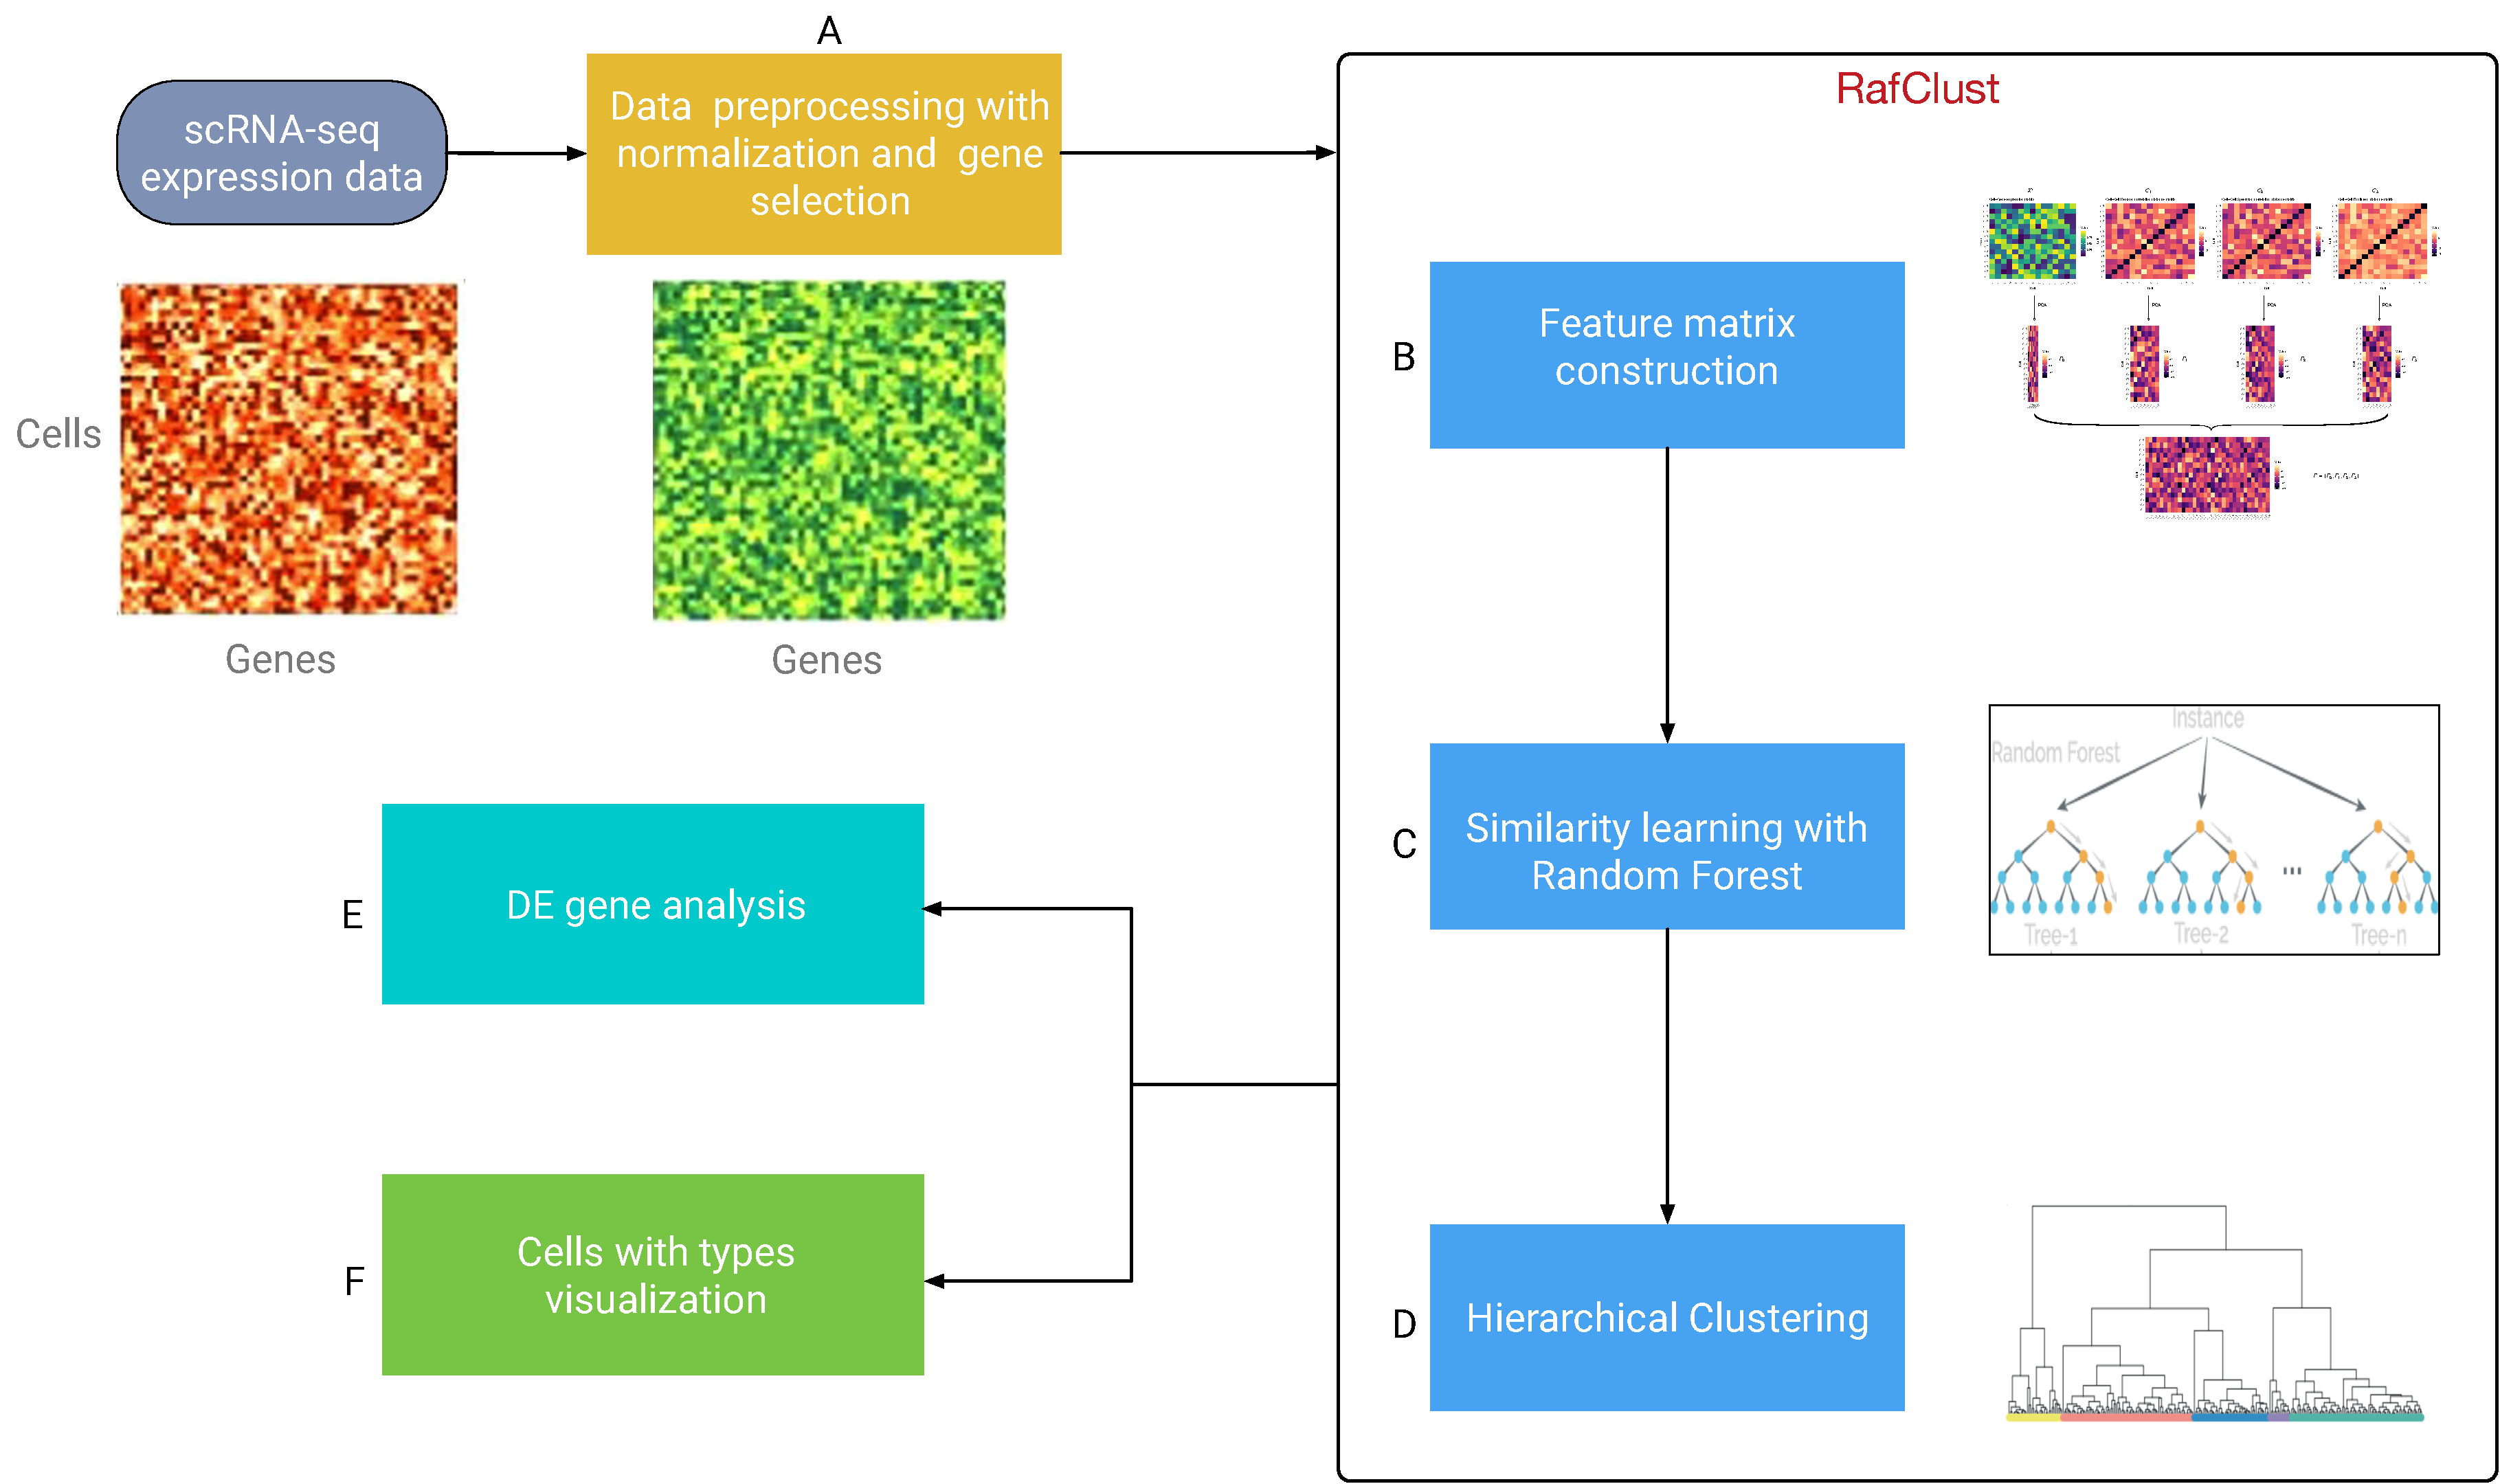
\includegraphics[width=0.95\textwidth]{flowchart-rafclust.pdf}
    \caption{RafClust~流程图。
    本图中的每个注释图代表了相应过程的输入或输出可视化。输入的是~scRNA-seq~表达数据二维矩阵,其中行代表细胞,列代表基因。
    (A)~用输入的表达数据进行数据预处理,输出的是一个归一化和列的维度缩减的矩阵。
    (B-D)~RafClust~的核心程序。
    (B)~利用表达数据构造特征矩阵。
    (C)~利用随机森林算法来学习细胞与细胞的相似性矩阵。
    (D)~利用层次聚类来对细胞进行聚类。
    (E)~对不同类型的细胞进行不同的差异基因分析,从而得到细胞类型的特异基因。
    (F)~细胞表达数据与其类型可视化,在基于~t-SNE~的二维图中不同的颜色代表不同的细胞类型。
    }
    \label{fig:rafclust}
\end{figure}

\subsubsection{数据规范化和基因选择}
\label{subsec:datapreprocessing} 

我们假设归一化的~$n$~个细胞的基因表达数据~(观测值), 每个细胞含有~$p$~个基因(特征),
组成一个~$n \times p$~的表达式矩阵~$X=\left(x_{1}, x_{2}, \ldots, x_{n} \right)^ T$。
其中~$x_{i}$~表示~$p$~基因在细胞~$i$~中的表达值。
$x_{i}=\left(x_{i1}, x_{i2},\ldots, x_{ip} \right)$。
矩阵~$X$~在加上~1~的伪数~(pseudo-count)~后进行对数变换,即~$X^{\prime} = log_2 (X + 1)$。
然后,如果基因在细胞总数中的表达低于一个预定频率~$\beta$,则该基因会被过滤掉。
默认情况下,~$\beta$~设置为~0.06~\cite{kiselev2017sc3}。 
基因过滤的动机是,除了保守的基因外,其它一些很普通的甚至是低表达的基因往往对细胞的聚类没有贡献。

\subsubsection{细胞类型识别}
\label{subsec:rafclust} 
为了从稀有细胞集合中确认不同的细胞类型,我们提出了一种无监督的基于随机森林的相似性学习算法,命名为~RafClust。
类似于其它的许多方法~\cite{kiselev2017sc3,pouyan2018random,mohammadi2018geometric,sinha2018dropclust,Srinivasan511626,Li530378,zheng2019sinnlrr},
RafClust~也是两个步骤的方法,
第一个步骤是我们使用随机森林进行相似度学习~(相似性学习步骤,~similarity learning),
第二个步骤中我们使用层次聚类~(聚类步骤,~clustering)。
在相似度学习步骤中,一个非常关键的预处理程序是特征矩阵的构建。
稀有细胞~(rare cells)~与丰富细胞~(abundant cells)~不同,我们将使用细胞和细胞的尽量多的不同类型的相似性,来充分刻画稀有细胞的本性特征。
因此,在基于基因过滤后的表达矩阵~$X^{\prime}$~上,
我们利用欧几里德~(Euclidean)、皮尔逊~(Pearson)~和斯皮尔曼~(Spearman)~指标分别计算出三种不同的细胞-细胞距离矩阵~$\{C_1, C_2, C_3\}$。
然后将主成分分析~PCA~应用于每个距离矩阵,也应用于~$X^{\prime}$~上,来减少数据维度的同时也去除其本能噪声。
每个矩阵中信息量最大的成分由``elbow~法"~\cite{thorndike1953belongs}~保留,
这样就共计产生了~$\left\{ {F}_{i} \in \mathbb {R} ^ {n \times m_{i}} \right\}_{i = 0}^{3}$~四个矩阵。
最终的特征矩阵~$F$~由这些矩阵按行拼接组成, 行代表细胞, 列代表手工特征~(handcrafted features)\footnote{区分于现在比较流行的深度学习里的~auto-learned features}。
\begin{equation}
\label{lab:f}
{F} = ({F}_{0}, {F}_{1}, {F}_{2}, {F}_{3})
\end{equation}

$F$~中的列数~(维度)~(即特征总数~$\tilde {p} = \sum_{i = 1}^{k} m_{i}$)~与数据有关。
和细胞~$j$~现在用特征向量~$f_{i} \in \mathbb {R} ^ {\tilde{p}}$~表示。
显然,$F$~既反应了细胞的自身表达值,也包含了细胞与其它细胞的相似性关系特征。
接着,我们利用特征矩阵~$F$~来进行基于随机森林~(RF)~的相似性学习。
图~\ref{fig:rafsim}~是一个示例,在大小为~$15 \times 15$~基因表达矩阵的数据集上来说明整个特征矩阵的构建步骤。

% \begin{figure}[!htbp]
%   \begin{adjustbox}{addcode={
%     \begin{minipage}{\width}}{
%         \caption{一个有~15~个细胞和每个细胞~15~个基因的示例数据集中手动制作的特征矩阵构造。
%         最终的特征矩阵~$F$~在这个示例中是~$15\times34$~维度大小的。}
%         \label{fig:rafsim}
%     \end{minipage}},rotate=90,center}
%     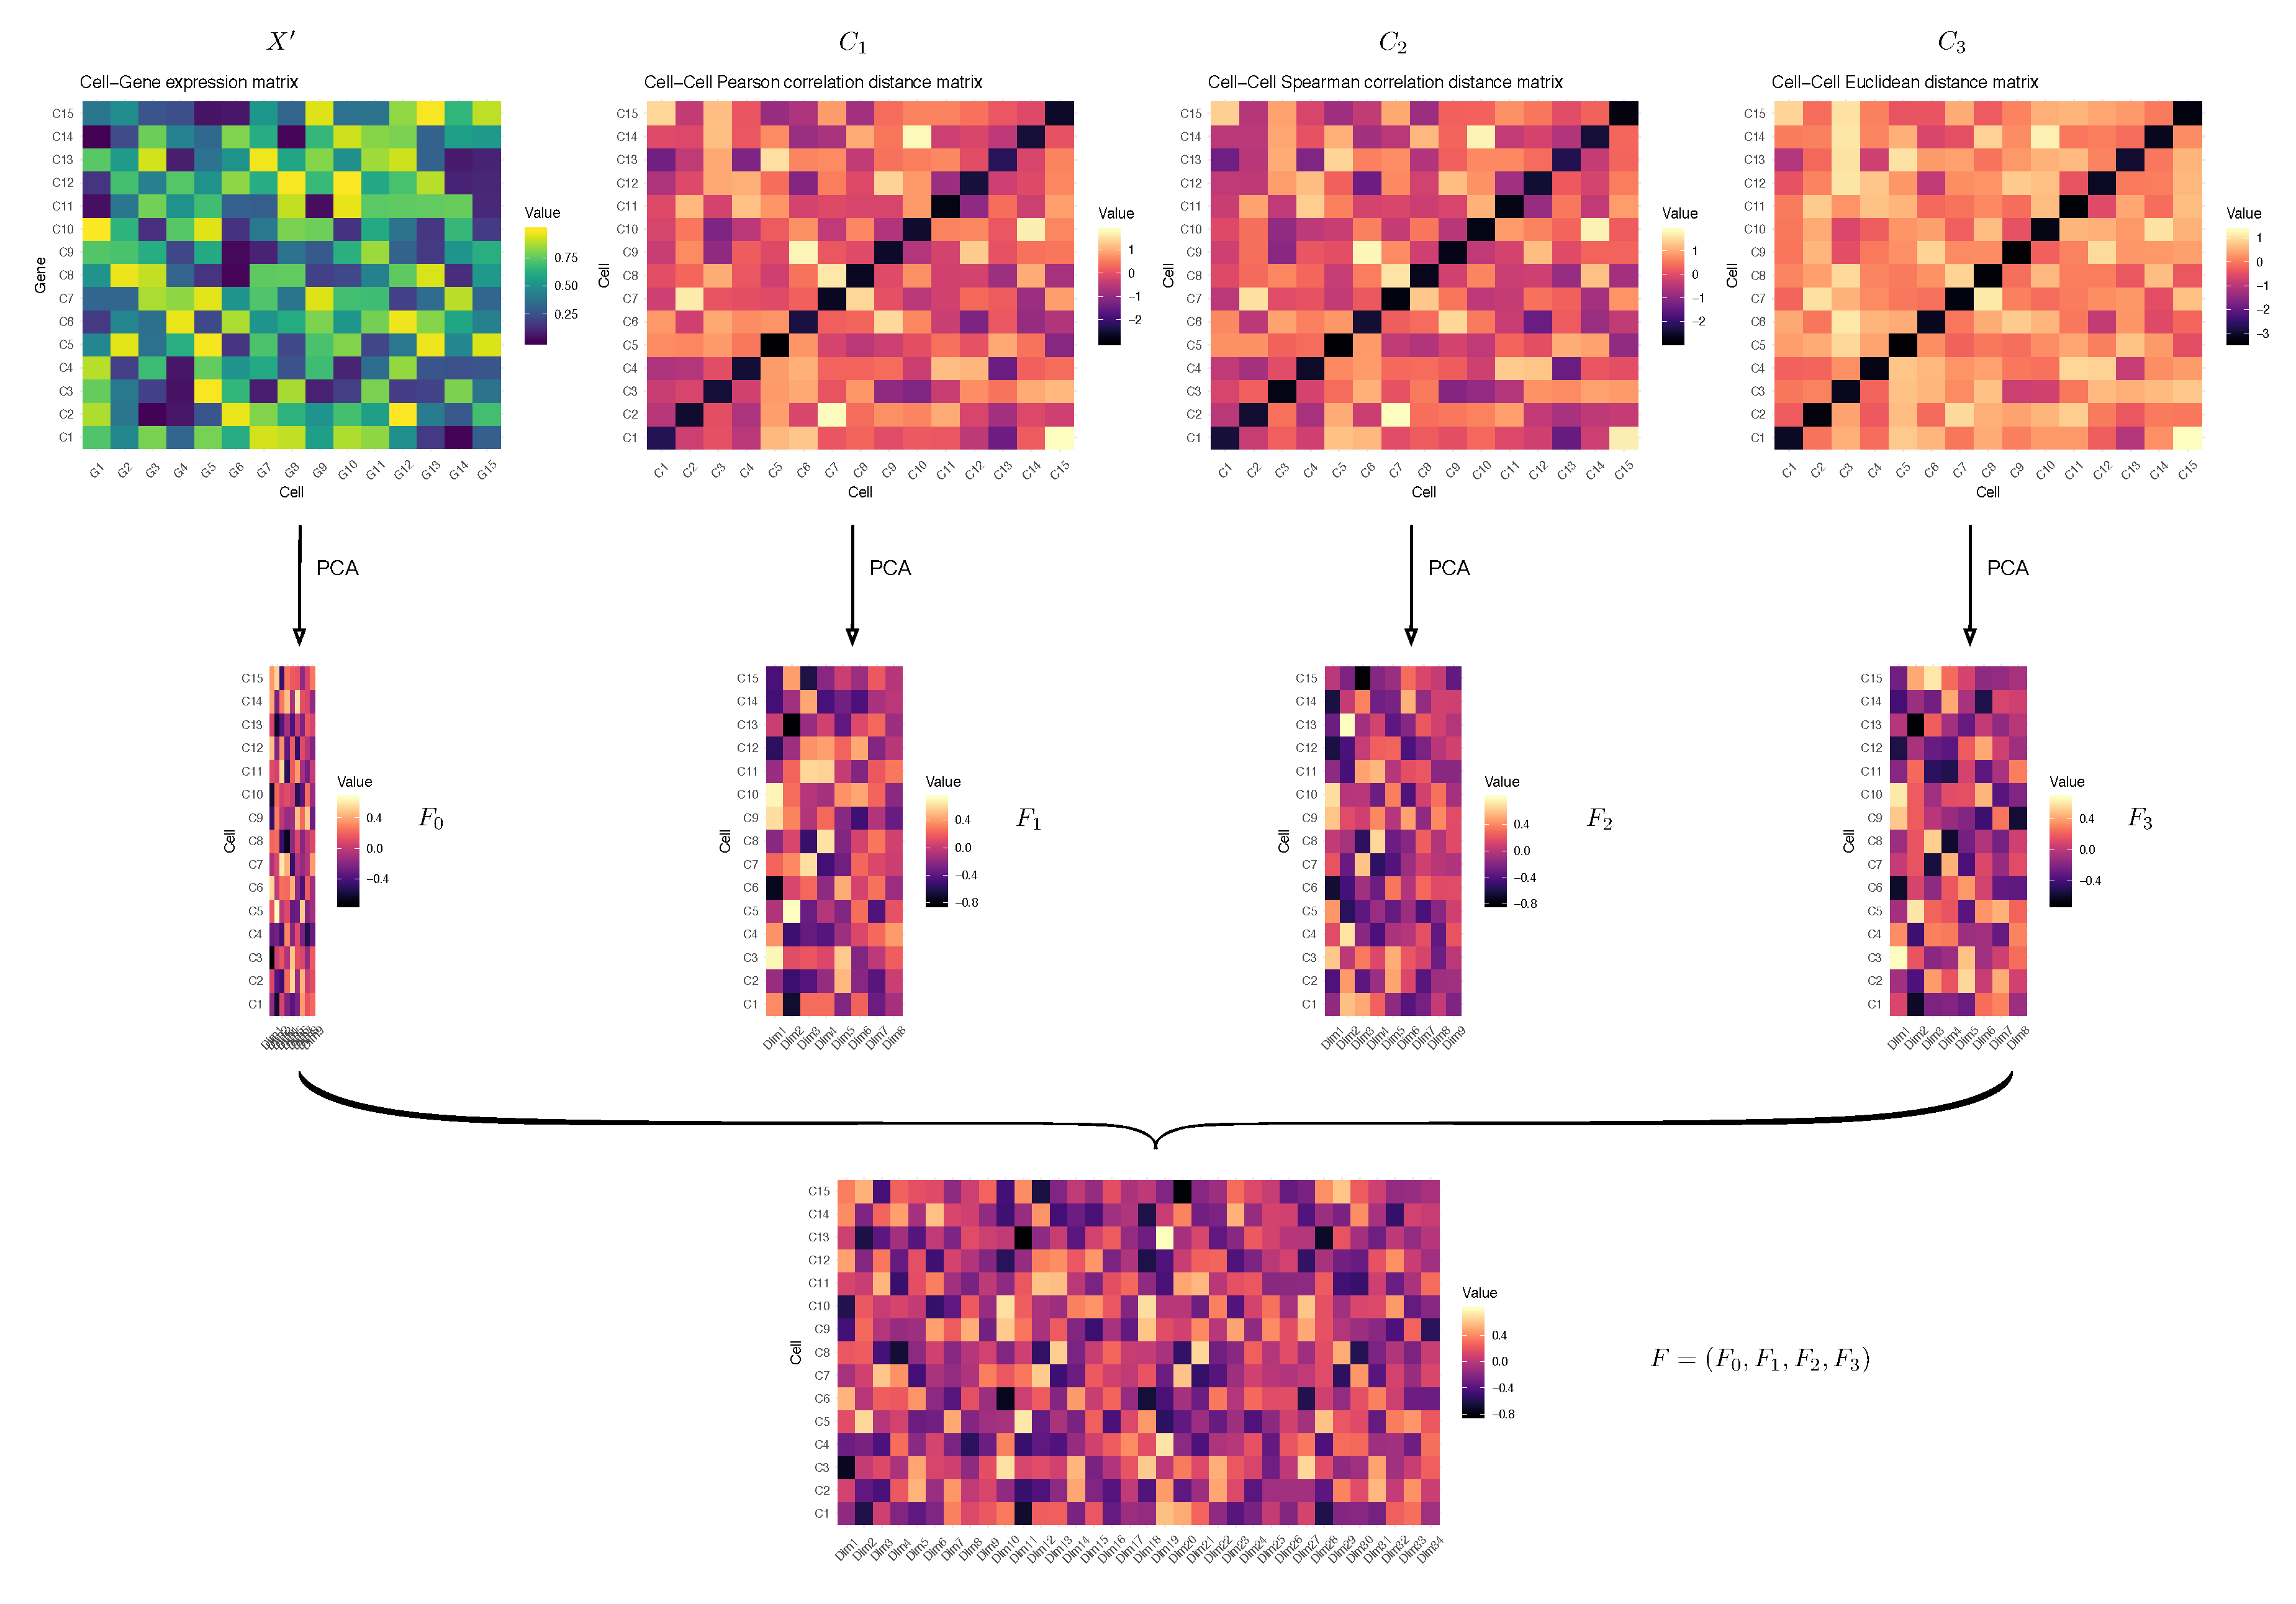
\includegraphics[scale=.42]{rafsim.pdf}%
%   \end{adjustbox}
% \end{figure}
\begin{figure}[!htbp]
    \centering
    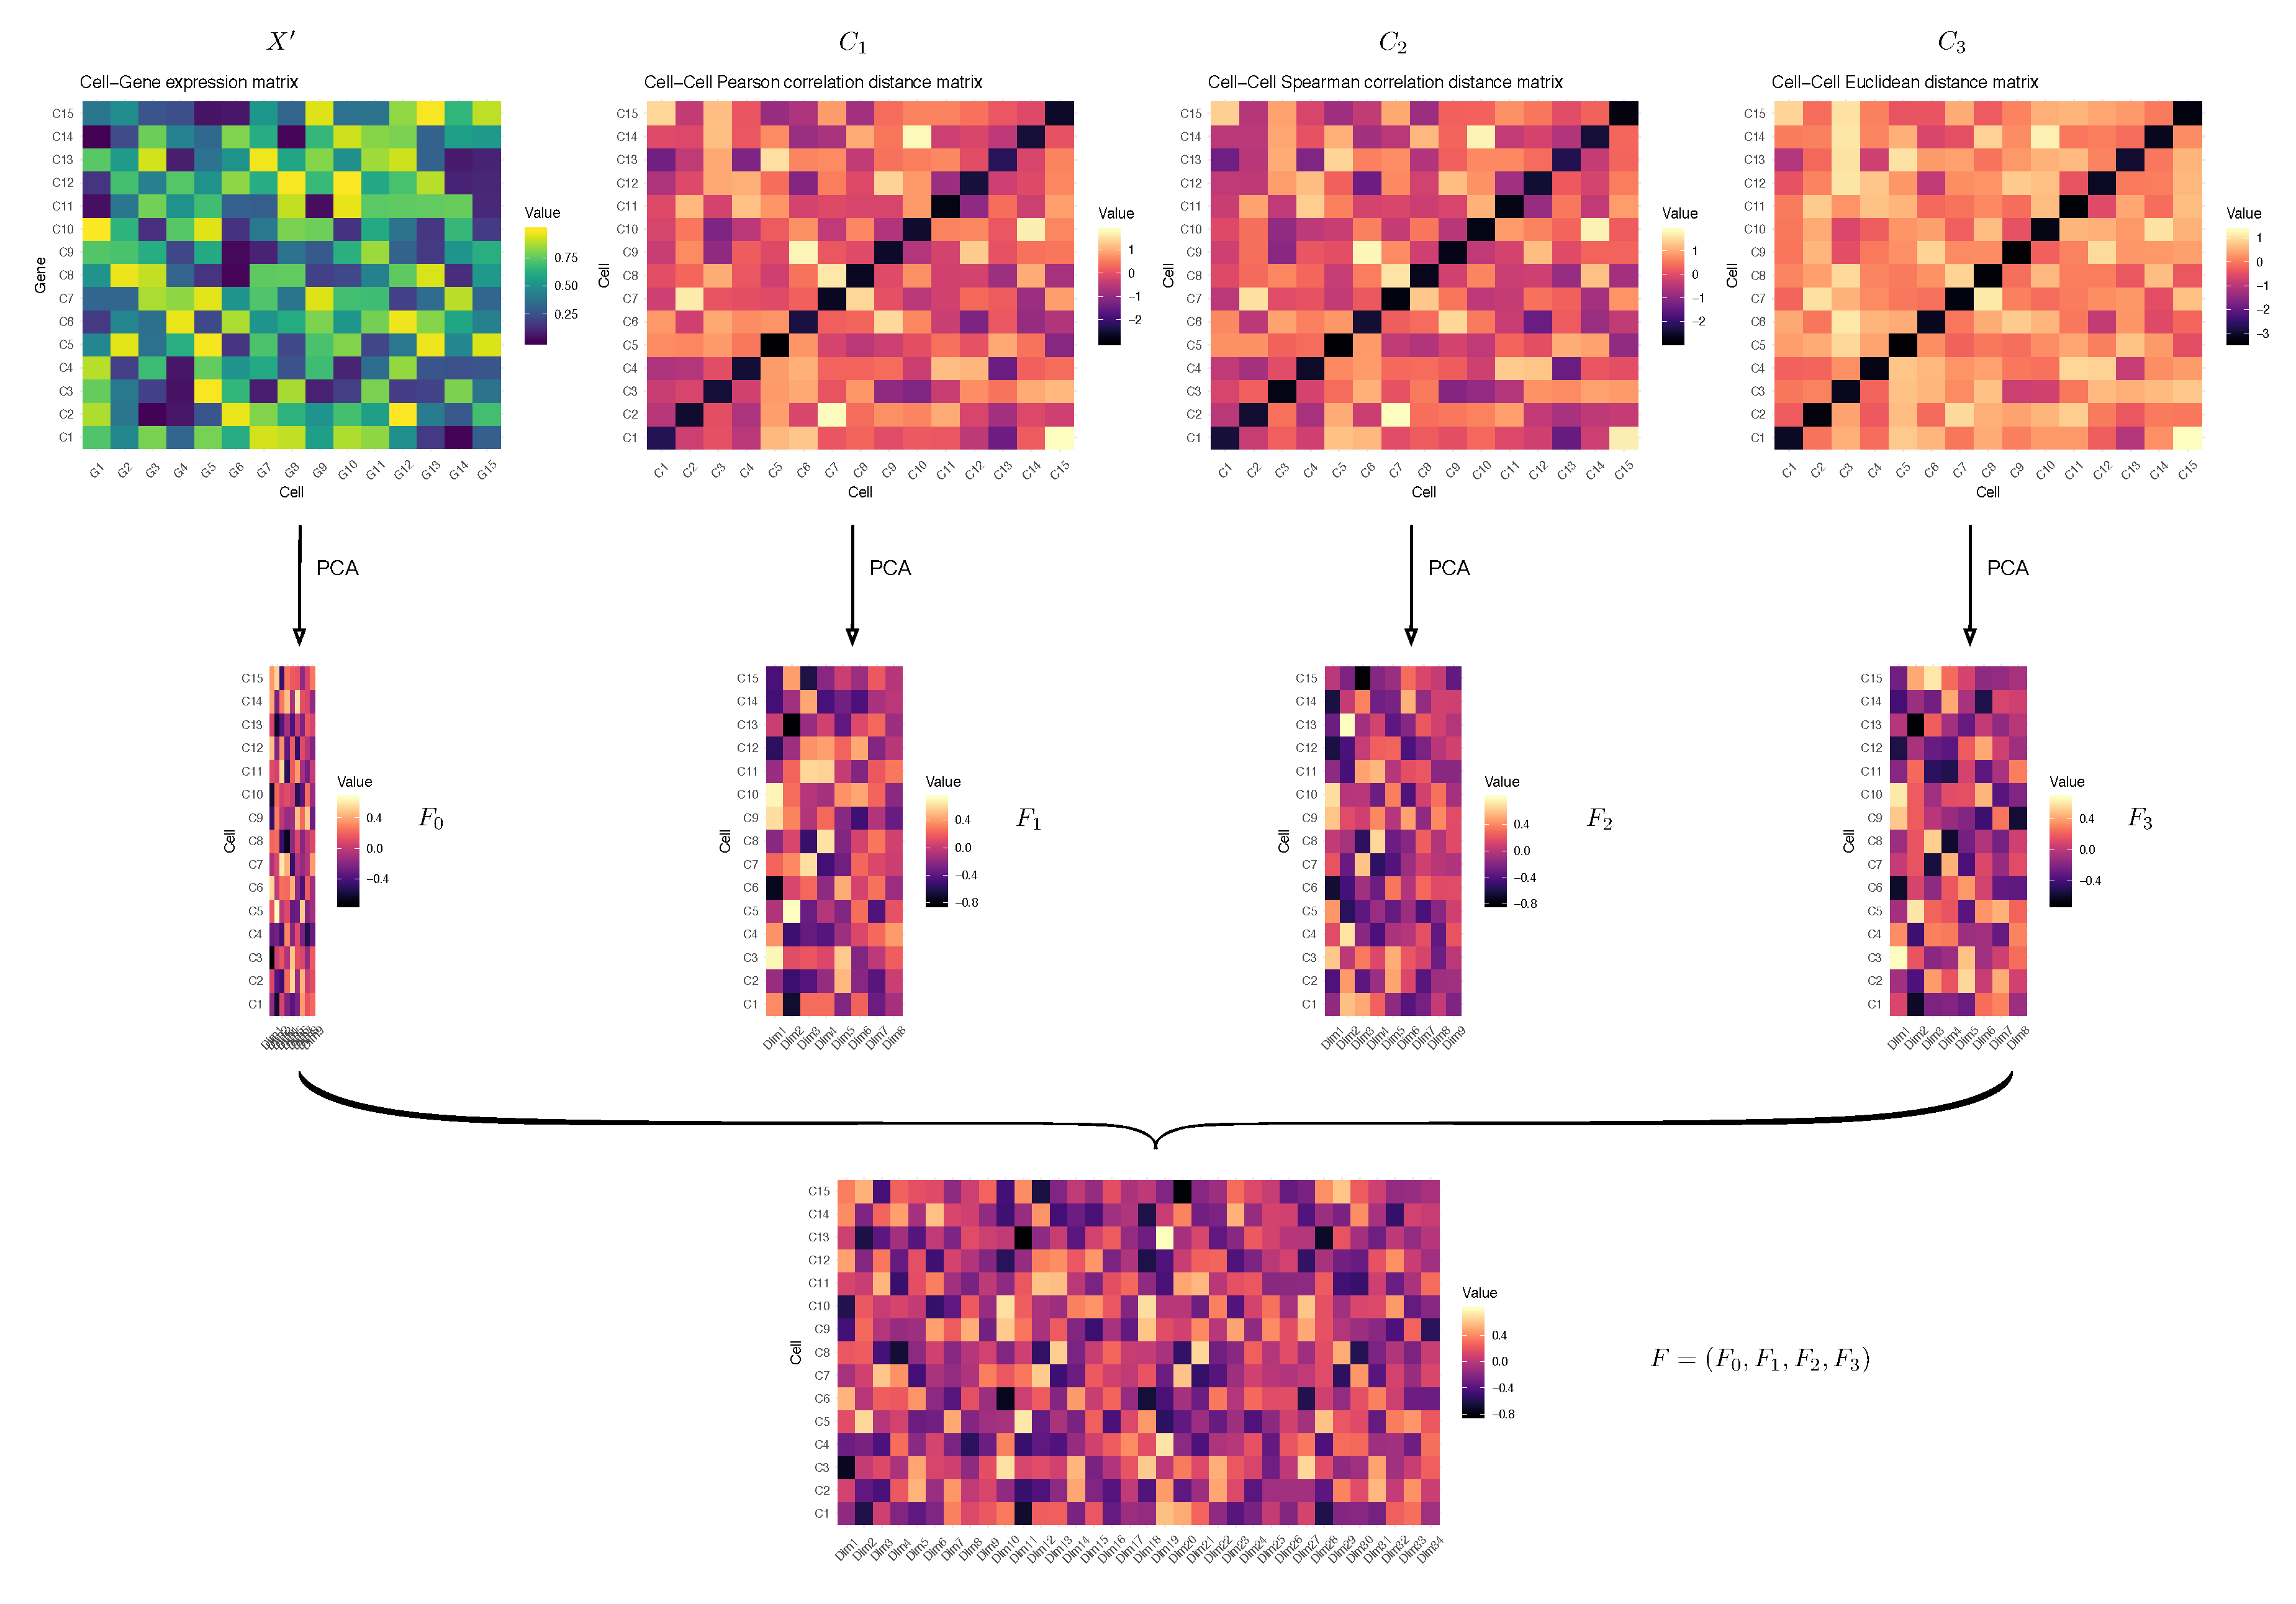
\includegraphics[width=0.9\textwidth]{rafsim.pdf}
    % \caption{Illustration of the hand-crafted feature matrix construction in a toy dataset with 15 cells and 15 genes. 
    % The final feature matrix $F$ is in a $15 \times 34$ shape in this case}
    \caption{
        一个有~15~个细胞和每个细胞~15~个基因的示例数据集中手动制作的特征矩阵构造。
        最终的特征矩阵~$F$~在这个示例中是~$15\times34$~维度大小的。
    }
    \label{fig:rafsim}
\end{figure}

RF~(随机森林,~Random Forest)~是一种应用非常广泛的基于决策树的分类和回归方法~\cite{breiman2001random}。
另外,它也可以用无监督的方式来推断对象之间的相似性~\cite{shi2006unsupervised,breiman2011manual,pouyan2018random}。
另外,基于~RF~的相似性学习方法很容易适应于并行计算,
对离群值具有鲁棒性,内在具有特征选择的特性,这三个特点特别适合用来分析高维和噪声数据,
特别是类似于单细胞~RNA~测序图谱数据。
我们按照以下步骤来学习细胞-细胞的相似性。
在选择一个单一的特征~$j$~(特征矩阵~$F$~中的第~$j$~列)~后, 
我们使用围绕质心点进行划分的算法~PAM~(partitioning around medoids),估计类别的数量并得到对应于类别的伪标签。
与~K-means~聚类算法相比,~PAM~对孤立点不敏感。
%我们直接使用~R~包~fpc~\cite{package-fpc}中的~\textit{pamk}~函数来获取该特征~$j$~的向量中的类标签。
然后,我们从~$F$~中去掉第~$j$~列,并且使用~RF~对缩减后的数据集~$F_{-j}$~进行对伪标签的回归学习。
让~$f_p$~表示~$F_{-j}$~的第~$p$~行,
如果~RF~包含~$N$~颗树,并定义~$nt(f_p,f_q)$, 作为通过同一片叶子对细胞~$f_p$~和~$f_q$~进行归类的树的数量。
基于~RF~的~$n \times n$~相似度矩阵~$S_j$~是通过以下方式定义:
$S_{j_{pq}} = nt(f_p,f_q) / N, 1 \le p,q \le n$。
%我们使用~R~包~randomforest~\cite{package-randomforest},其默认森林大小为~500~棵,即~$N=500$。
对所有的~$\tilde{p}$~特征重复这个过程,得到~$\tilde{p}$~相似度矩阵~$S_j$,$j=1,2,\ldots,\tilde{p}$。
通过对所有~$S_j$~进行平均,得到最终的细胞-细胞相似度矩阵~$S$,
并通过~$D=1-S$~得到距离矩阵~$D$。

接下来,对距离矩阵~$D$,使用层次聚类中的平均连锁聚类方法~(average linkage clustering)~来对细胞进行聚类,
使用了来自~R~包~dynamicTreeCut~\cite{langfelder2007defining,package-dynamicTreeCut}~的~\textit{cutreeDynamic}~函数自动确定细胞的类别,
并为每个细胞分配正确的类标签。
另外,我们还提供了使用~R~包~dynamicTreeCut~中的~\textit{cutree}~函数来支持用户自定义细胞的类别数。

\subsubsection{差异基因分析}
\label{subsec:de}

使用~RafClust~得到了细胞的类别标签后,
我们采用~NODES~\cite{Sengupta049734}~这一快速的非参数化、差异化表达~(DE)~分析工具进行差异基因分析。
NODES~被证明比传统的基于批量细胞测序的差异分析方法~DESeq2~\cite{love2014moderated}、edgeR~\cite{robinson2010edger},
以及针对单细胞的差异表达分析方法~scde~\cite{kharchenko2014bayesian}~和~Wilcoxon~秩和检验~(Wilcoxon rank sum test)~都有效~\cite{Sengupta049734}。
以~0.05~作为~FDR~(False Discovery Rate)~的阈值,~FC~(fold change)~变化(也就是两个组间表达量的比值)~阈值默认为~log2(5)。
在~DE~基因中,在特定类中相对于其余各类显著上调的基因被命名为细胞类型特异基因。


\subsection{实验结果}

\subsubsection{数据集}
\label{subsec:datasets} 

为了测试~RafClust~在单细胞聚类场景下的性能,
我们使用了十个知名的~scRNA-seq~数据集上,细胞数目从小规模到中等规模不等。
每个数据集以第一作者的姓氏命名如下: 
Biase~\cite{biase2014cell},
Treutlein~\cite{treutlein2014reconstructing}, 
Pollen~\cite{pollen2014low}, 
Kolod~\cite{kolodziejczyk2015single}, 
Usoskin~\cite{usoskin2015unbiased}, 
Darmanis~\cite{darmanis2015survey}, 
Goolam~\cite{goolam2016heterogeneity}, 
Li~\cite{li2017reference},
Tasic~\cite{tasic2016adult}, 
Zeisel~\cite{zeisel2015cell}。
这十个数据集可以在~\url{https://hemberg-lab.github.io/scRNA.seq.datasets}~上获取, 
每个数据集的详情介绍如表~\ref{tbl:clusteringdatasets}~所示。

\begin{table}[!htbp]
  \centering
  \caption{
      %Overview of the  benchmark  datasets for the clustering performance comparison of RafClust with the other competing methods
      RafClust~与其它竞争方法的聚类性能比较所使用的基准数据集概述
      }
  \label{tbl:clusteringdatasets}
  \resizebox{\columnwidth}{!}{%
  \begin{tabular}{llllrrrr}
  \toprule
  Dataset   &Accession 	&Sequencing protocol &Units &\#Cells &\#Genes	&\#Populations  & References \\
  \midrule
  Biase     &GSE57249     &SMARTer    &FPKM   &56	     &25 734     &5         &\cite{biase2014cell}\\
  Treutlein &GSE52583  	&SMARTer   	&FPKM  	&80      &23 271     &5 		&\cite{treutlein2014reconstructing}\\
  Pollen    &SRP041736 	&SMARTer   	&TPM   	&301     &23 730     &11 		&\cite{pollen2014low} \\
  %Patel     &GSE57872     &Smart-Seq 	&TPM   	&430     &5 948      &5			&\cite{patel2014single}\\
  Kolod     &E-MTAB-2600  &SMARTer    &CPM    &704     &38 616     &3         &\cite{kolodziejczyk2015single}\\
  Usoskin   &GSE59739  	&STRT-Seq  	&RPM   	&622     &25 334     &11 		&\cite{usoskin2015unbiased}\\
  Darmanis  &GSE67835  	&SMARTer    &CPM    &466     &22 088     &9         &\cite{darmanis2015survey}\\
  Goolam    &E-MTAB-3321  &Smart-Seq2	&CPM  	&124     &41 480     &5			&\cite{goolam2016heterogeneity}\\
  Li     	  &GSE81861  	&SMARTer    &CPM   &561     &55 186      &9         &\cite{li2017reference}\\
  Tasic     &GSE71585     &SMARTer    &RPKM   &1 679   &24 057     &18        &\cite{tasic2016adult}\\
  Zeisel    &GSE60361     &STRT-Seq  	&UMI   	&3 005   &19 972     &9			&\cite{zeisel2015cell}\\
  \bottomrule                   
  \end{tabular}
  }
\end{table}


\subsubsection{评价指标}
聚类的效果是使用真实的类别标签~$L_T$~和估计的类别标签~$L_E$~之间的相似性来衡量,
使用的是调整后的~Rand~指数~(Adjusted Rand index,~ARI)~\cite{hubert1985comparing,wu2005dynamic}:
\begin{equation}
\label{eq:ARI}
\resizebox{0.4\textwidth}{!}{$
    ARI(L_E,L_T)=\frac{\sum_{}{}_{e,t} \begin{pmatrix}n_{et}\\ 2\end{pmatrix} - \begin{bmatrix}  \sum_{}{}_{e} \begin{pmatrix}n_{e}\\ 2\end{pmatrix}\sum_{}{}_{t} \begin{pmatrix}n_{t}\\ 2\end{pmatrix}  \end{bmatrix} / \begin{pmatrix}n\\ 2\end{pmatrix} 
    }{\frac{1}{2}\begin{bmatrix}
    \sum{}{}_e\begin{pmatrix}n_{e}\\ 2\end{pmatrix} + \sum{}{}_t\begin{pmatrix}n_{t}\\ 2\end{pmatrix}
    \end{bmatrix} - \begin{bmatrix}
    \sum{}{}_e\begin{pmatrix}n_{e}\\ 2\end{pmatrix} \sum{}{}_t\begin{pmatrix}n_{t}\\ 2\end{pmatrix} 
    \end{bmatrix}/\begin{pmatrix}n\\ 2\end{pmatrix}}    
$}
\end{equation}
其中~$n$~是单细胞的总个数, 
$n_e$~和~$n_t$~分别是估计的类别~$e$~和真实的类别~$t$~中的单细胞数目; 
并且~$n_{et}$~是估计的类别~$e$~和真实的类别~$t$~共有的单细胞的数目。
ARI~的范围是~-1~到~1~,其中~1~表示估计的聚类与真实的聚类完全相同。
ARI~值越高,算法的聚类效果越好。

\subsubsection{实验结果分析}

为了测试~RafClust~的性能,
我们将其应用在十个知名的~scRNA-seq~数据集上~(数据详情见表~\ref{tbl:clusteringdatasets}),
将其~ARI~值与其它六种方法进行比较,
包括~RaceID2~\cite{grun2016novo}, CIDR~\cite{lin2017cidr}, SIMLR~\cite{wang2018simlr}, SAFE~\cite{yang2018safe}, RtsneKmeans~\cite{hartigan1979algorithm,maaten2008visualizing,van2014accelerating}, RAFSIL~\cite{pouyan2018random}。
这六种聚类方法均以~R~包的形式实现并公开了代码,它们的概述如表~\ref{supp-tbl:clustereringmethods}~所示。
通过将每种方法的聚类结果与每个基准数据集的细胞类型注释进行比较,计算出对应的~ARI~值。 
由于个别方法在代码中引入了随机函数和随机种子,使得运行结果有一定的随机性。
因此我们在每个数据集上对每个方法重复运行~5~次,结果中位数的~ARI~值如图~\ref{fig:rafari}~所示。
由图~\ref{fig:rafari}~可知,~RafClust~在~ARI~上优于其它六种方法。
我们还记录了这个对比实验每个方法在每个数据集上的执行时间~(图~\ref{fig:running-detail}),并将平均执行时间与其它基准方法进行比较,结果如图~\ref{fig:running-summary}~所示。
该实验是在运行~GNU Linux/Ubuntu 16.04~操作系统与~4.15.0-46-generic~内核的工作站上进行的,
硬件配置如下:~Intel(R) Xeon(R) CPU E5-2630 v4 @ 2.20GHz,~40~个核心,~256GB~内存。
由图~\ref{fig:running-summary}~可知,~RafClust~针对细胞规模从小型到中型的~scRNA-seq~数据集在计算效率上是可以接受的。

\begin{table}[!htbp]
  \centering
  \caption{
  %Overview of the benchmark clustering methods
  使用的聚类方法概览
  }
  \label{supp-tbl:clustereringmethods}
  \resizebox{\columnwidth}{!}{%
      \begin{tabular}{lll}
      \toprule
      Method                                                                     & Description                                                                                                                                                        & Reference \\
      \midrule
      CIDR (v0.1.5)                                                              & PCA dimension reduction based on zero-imputed similarities, followed by hierarchical clustering                                                                    & \cite{lin2017cidr}         \\
      \begin{tabular}[c]{@{}l@{}}RaceID2 (March 3, \\ 2017 version)\end{tabular} & K-medoids clustering based on Pearson correlation dissimilarities                                                                                                  & \cite{grun2016novo}        \\
      RtsneKmeans                                                                & \begin{tabular}[c]{@{}l@{}}t-SNE dimension reduction (initial PCA dim=50, t-SNE dim=3, perplexity=30) and K-means \\ clustering with 25 random starts\end{tabular} & \cite{hartigan1979algorithm, maaten2008visualizing,van2014accelerating}        \\
      SAFE (v2.1.0)                                                              & Ensemble clustering using SC3, CIDR, Seurat and t-SNE + K-means                                                                                                     & \cite{yang2018safe}         \\
      SIMLR                                                                      & An appropriate cell to cell distance metric by multi-kernel learning, followed by spectral clustering                                                                                                                                                          & \cite{wang2018simlr}         \\
      RAFSIL                                                                     & Random forest based cell to cell similary learning, followed by K-means or hierarchical clustering                                                                                                                                                              & \cite{pouyan2018random}        \\
      \bottomrule
  \end{tabular}
  }
\end{table}

\begin{figure*}[!htbp]
    \centering
    \begin{minipage}[b]{0.45\linewidth}
      \centering
      \centerline{
        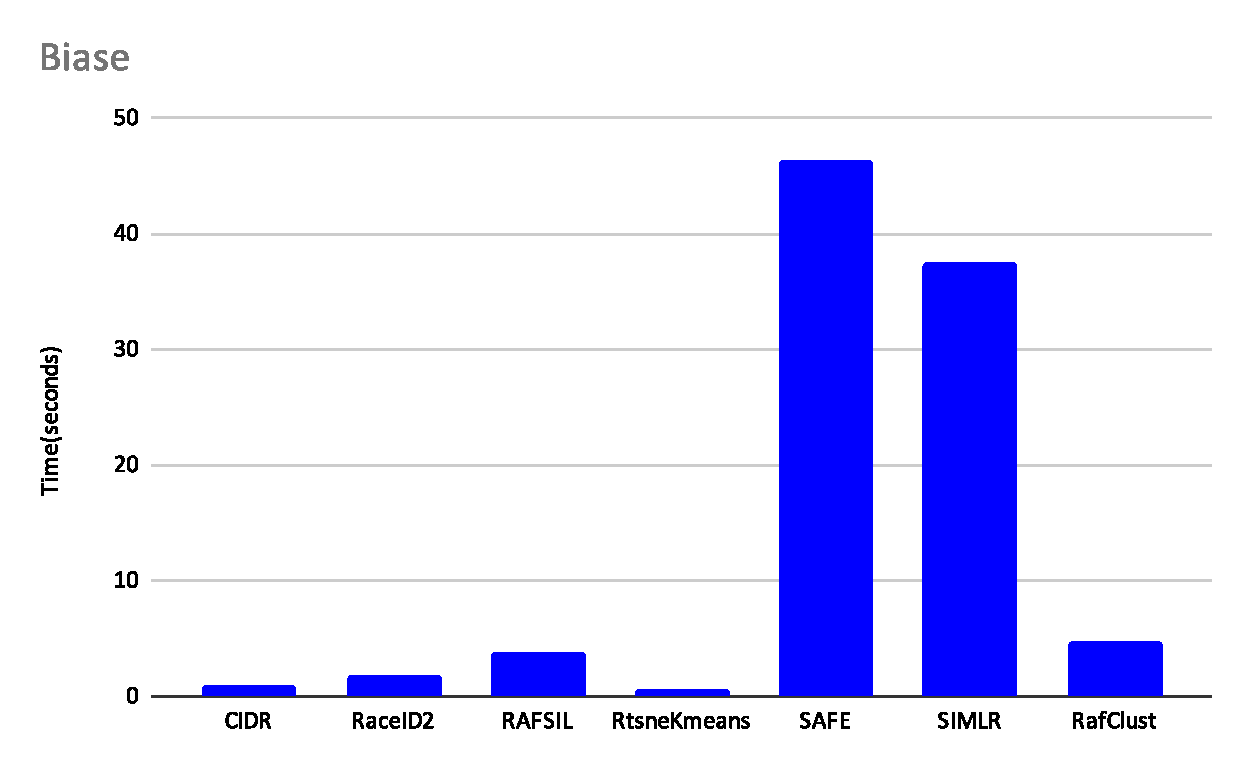
\includegraphics[width = \linewidth]{Biase.pdf}}
      \medskip  
    \end{minipage}
    \begin{minipage}[b]{0.45\linewidth}
      \centering
      \centerline{
        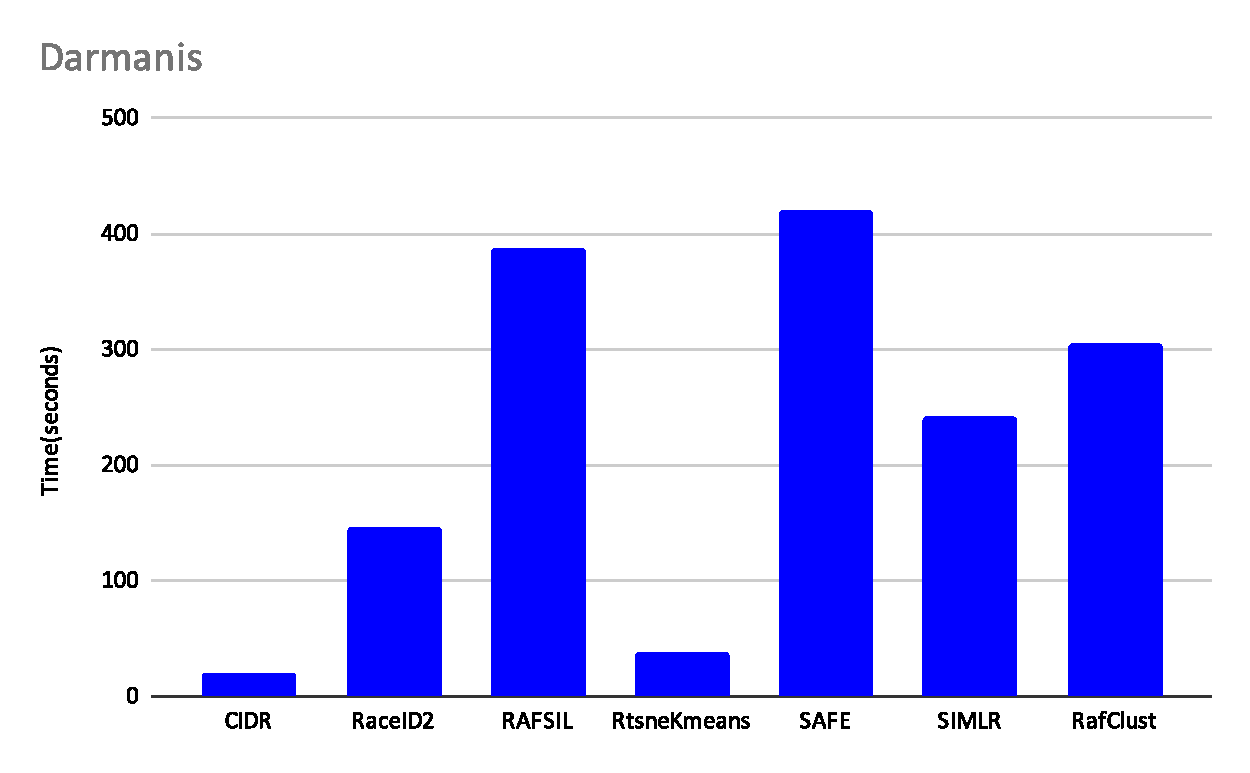
\includegraphics[width =\linewidth]{Darmanis.pdf}}
      \medskip  
    \end{minipage}
      \begin{minipage}[b]{0.45\linewidth}
      \centering
      \centerline{
        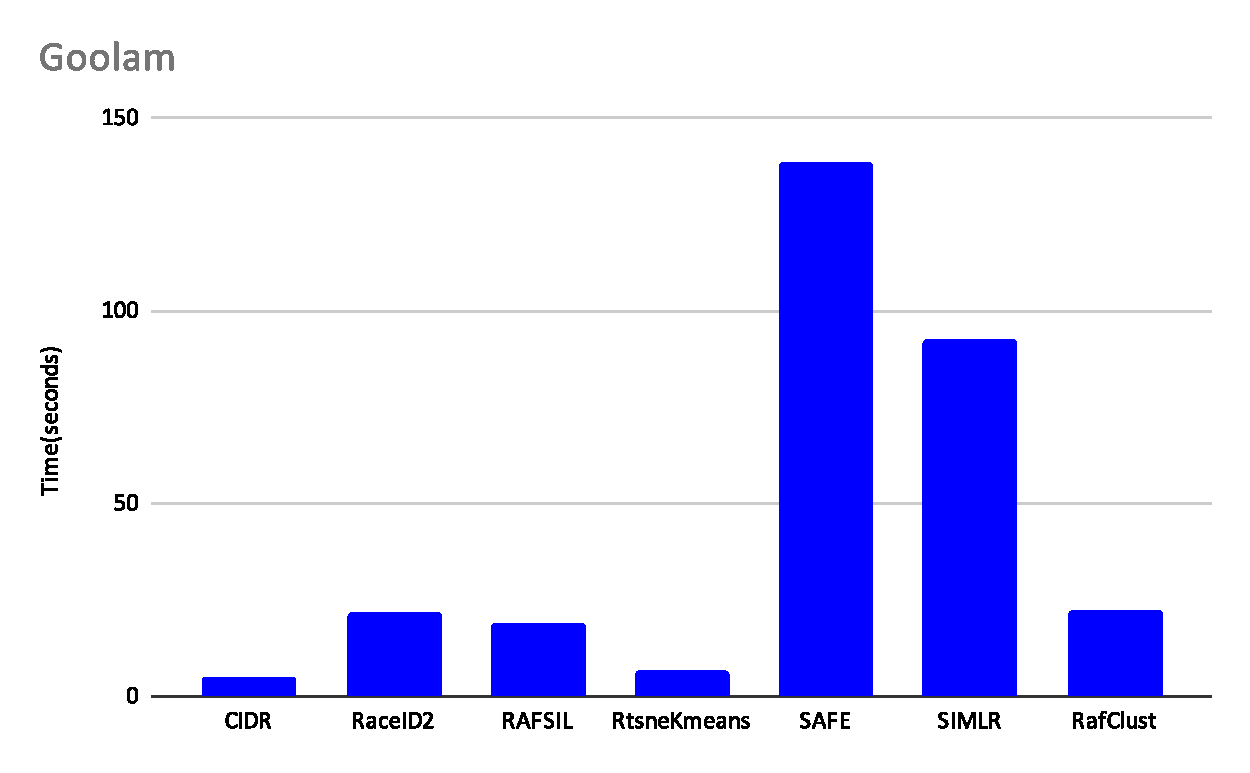
\includegraphics[width = \linewidth]{Goolam.pdf}}
      \medskip  
    \end{minipage}
    \begin{minipage}[b]{0.45\linewidth}
      \centering
      \centerline{
        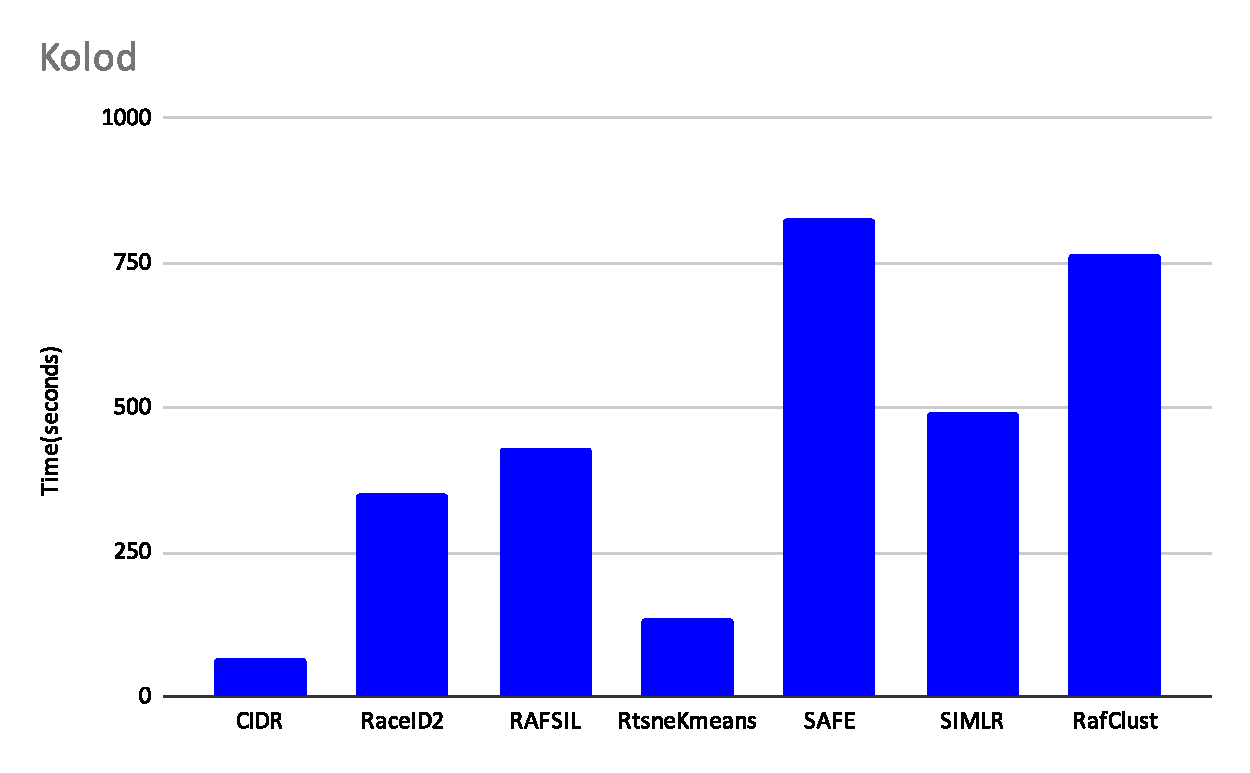
\includegraphics[width =\linewidth]{Kolod.pdf}}
      \medskip  
    \end{minipage}
    \begin{minipage}[b]{0.45\linewidth}
        \centering
        \centerline{
          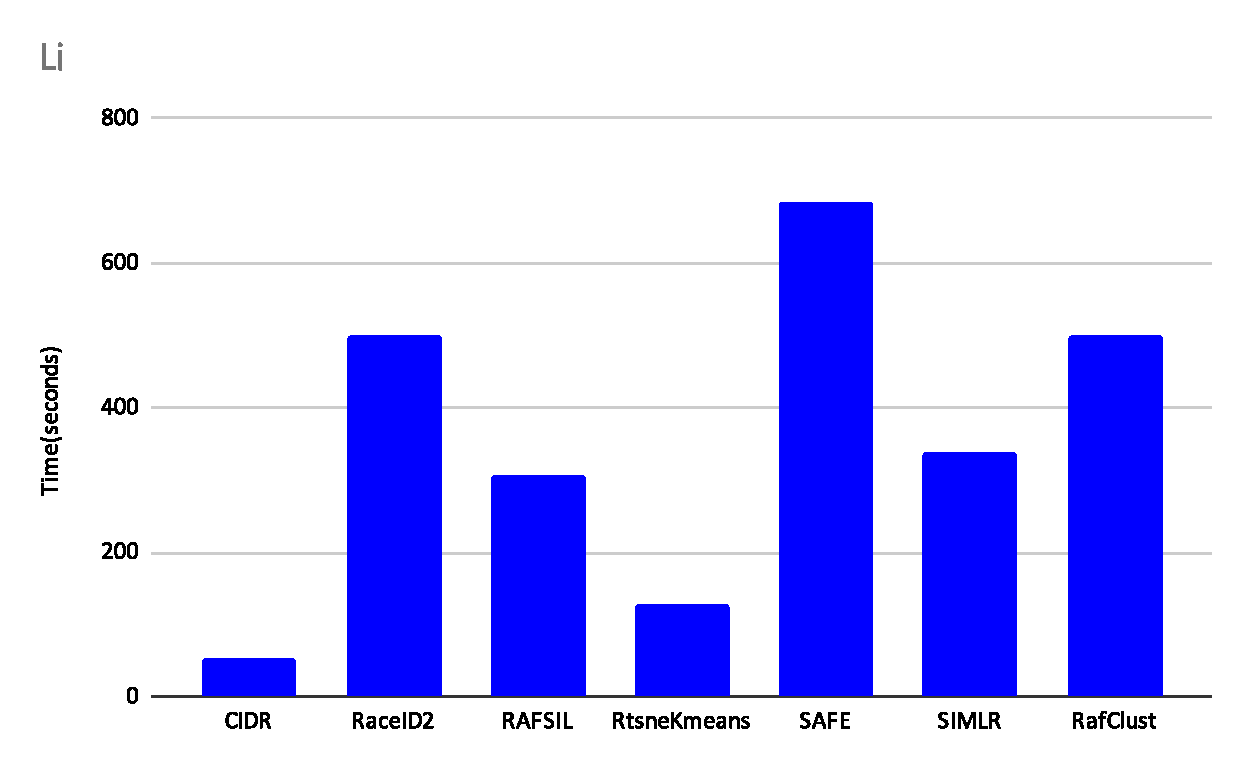
\includegraphics[width =\linewidth]{Li.pdf}}
        \medskip  
      \end{minipage}
      \begin{minipage}[b]{0.45\linewidth}
        \centering
        \centerline{
          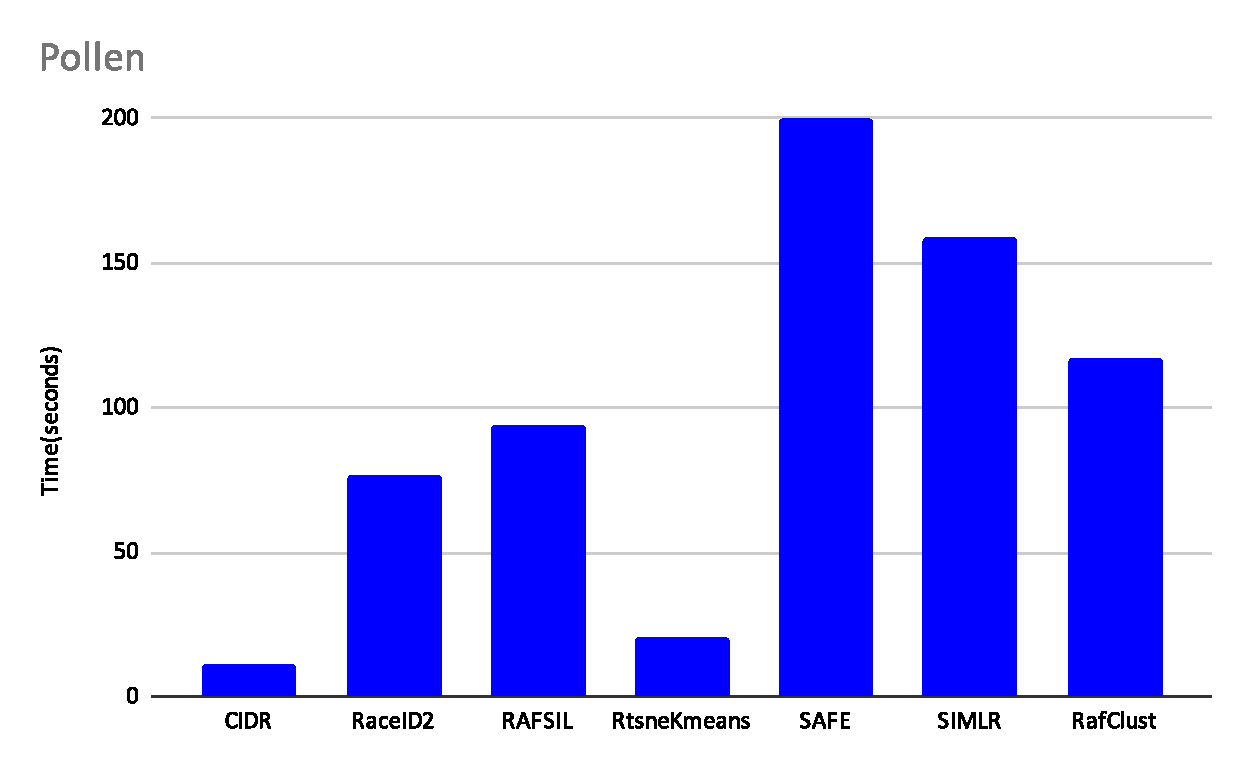
\includegraphics[width =\linewidth]{Pollen.pdf}}
        \medskip  
      \end{minipage}
      \begin{minipage}[b]{0.45\linewidth}
        \centering
        \centerline{
          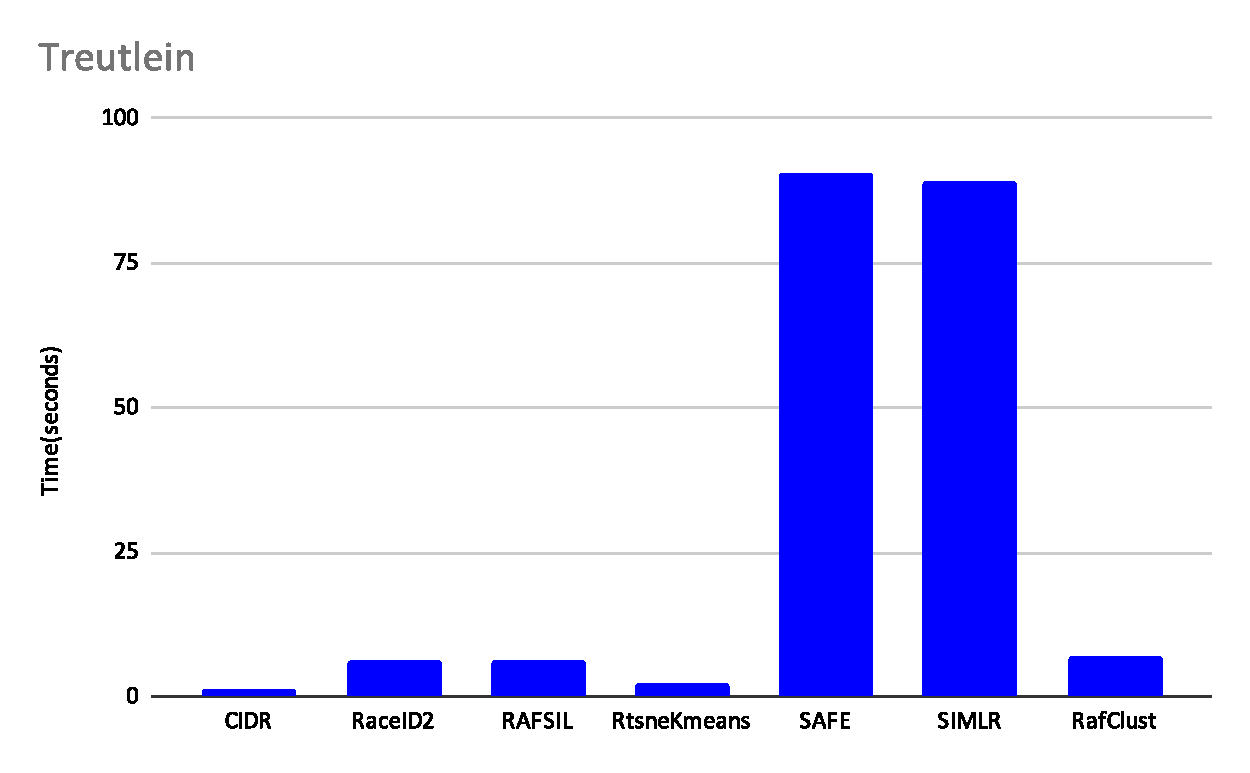
\includegraphics[width =\linewidth]{Treutlein.pdf}}
        \medskip  
      \end{minipage}
      \begin{minipage}[b]{0.45\linewidth}
        \centering
        \centerline{
          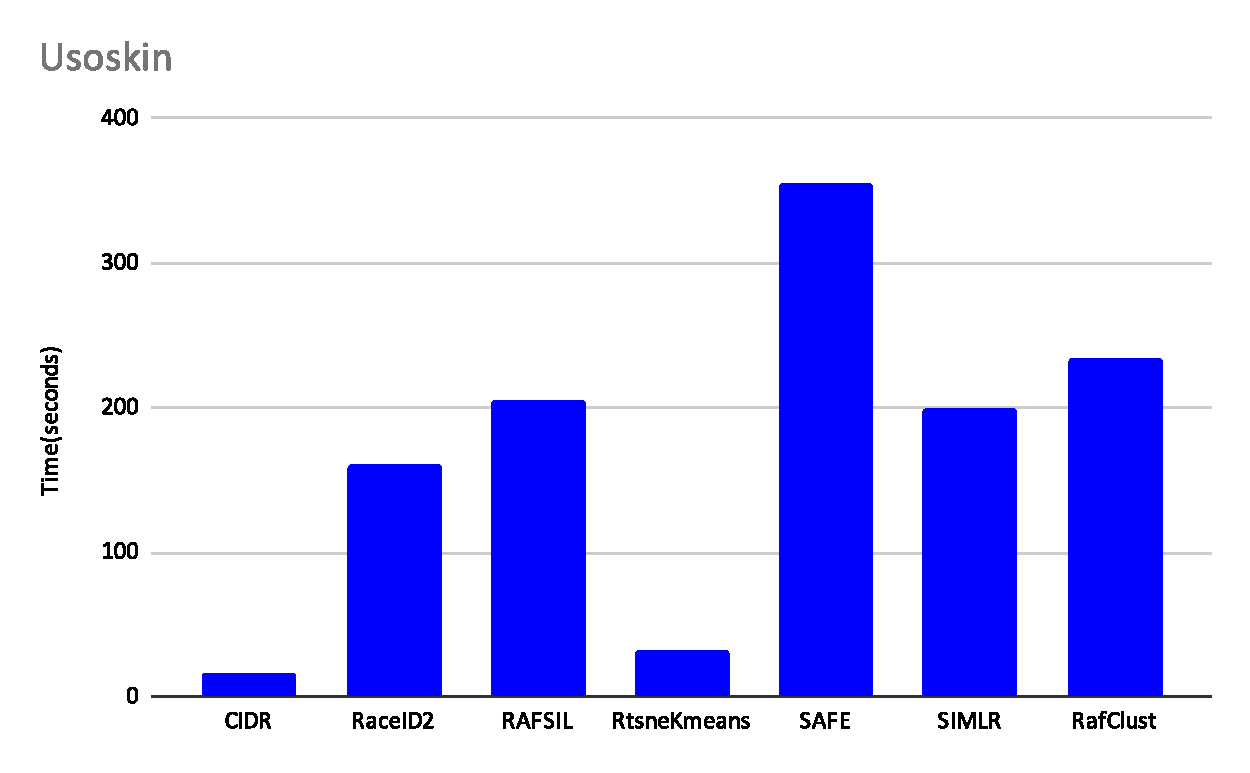
\includegraphics[width =\linewidth]{Usoskin.pdf}}
        \medskip  
      \end{minipage}
      \begin{minipage}[b]{0.45\linewidth}
        \centering
        \centerline{
          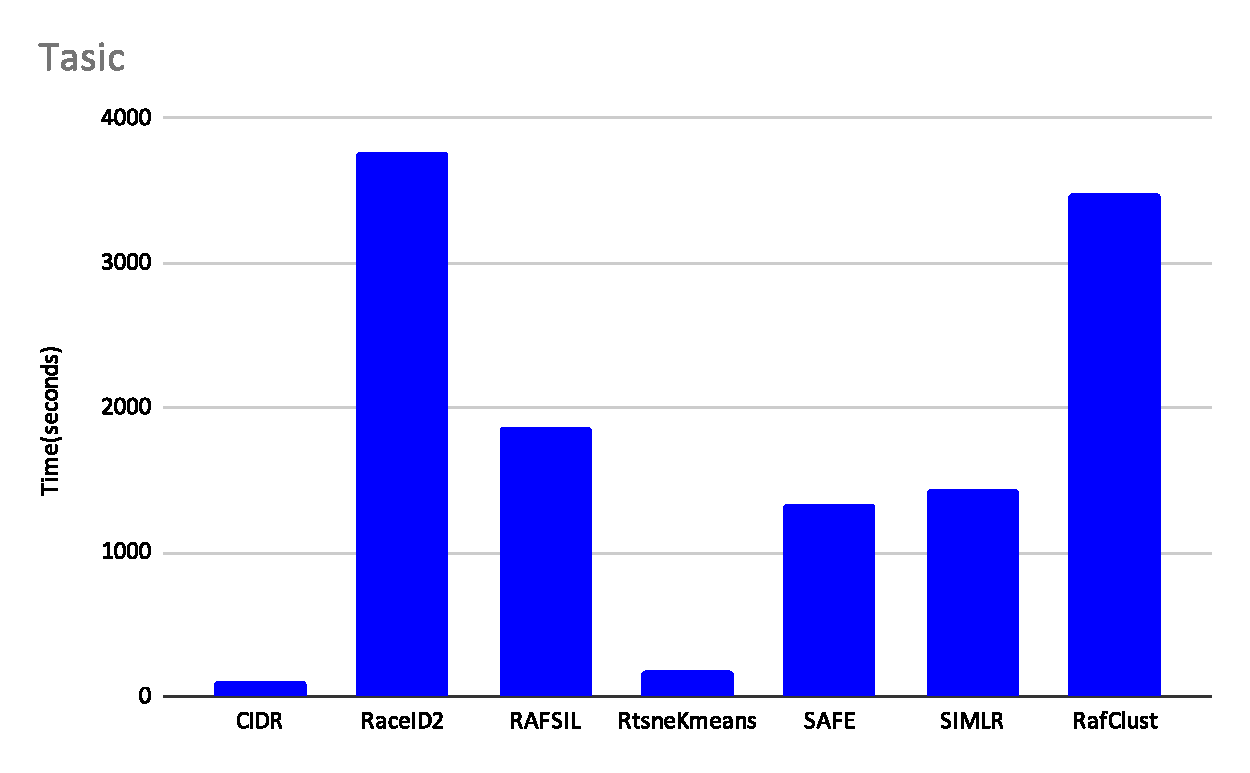
\includegraphics[width =\linewidth]{Tasic.pdf}}
        \medskip  
      \end{minipage}
      \begin{minipage}[b]{0.45\linewidth}
        \centering
        \centerline{
          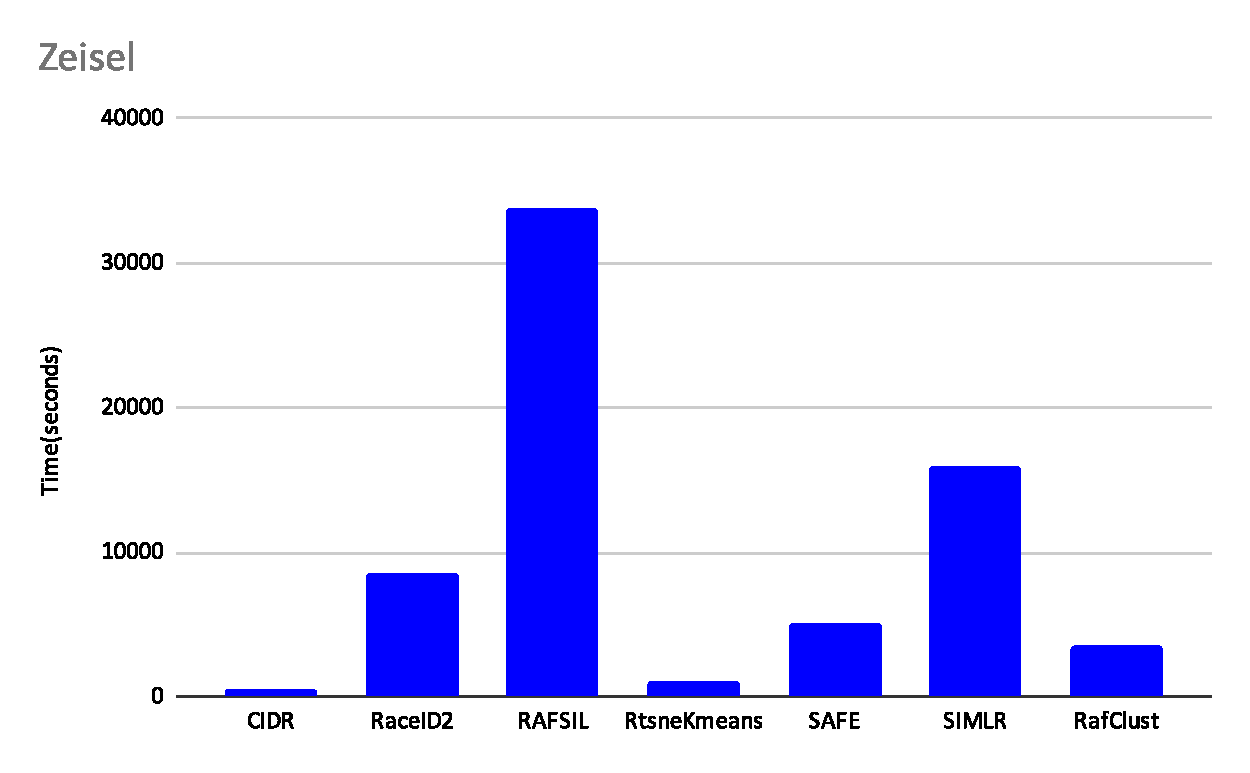
\includegraphics[width =\linewidth]{Zeisel.pdf}}
        \medskip  
      \end{minipage}
    \caption{
    RafClust~与其它六种方法在~10~个数据集上的中位数运行时间示意图。
    }
    \label{fig:running-detail}
    \vspace{-0.5em}
  \end{figure*}
 
  \begin{figure}[!htbp]
    \centering
    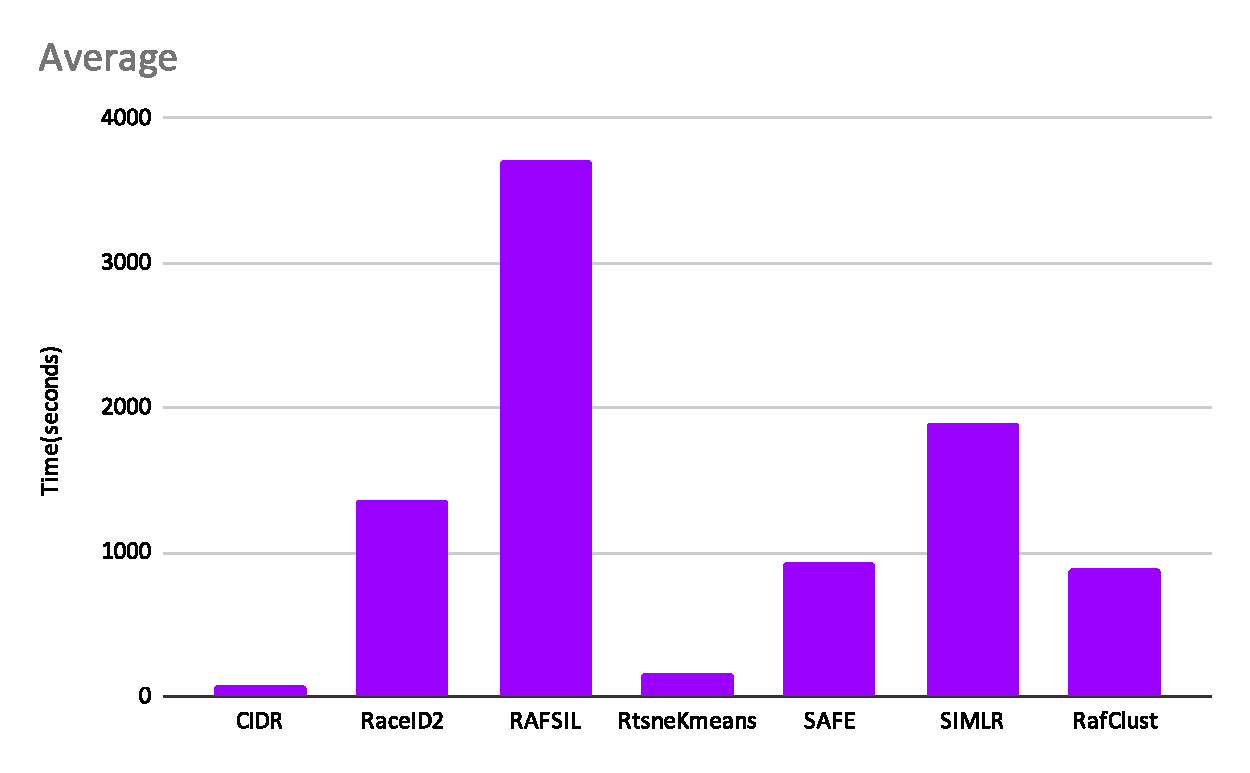
\includegraphics[width=0.9\textwidth]{Average.pdf}
    \caption{
    RafClust~与其它六种方法在~10~个数据集上的中位数运行时间示意图。
    }
    \label{fig:running-summary}
\end{figure}

\begin{figure}[!htbp]
    \centering
    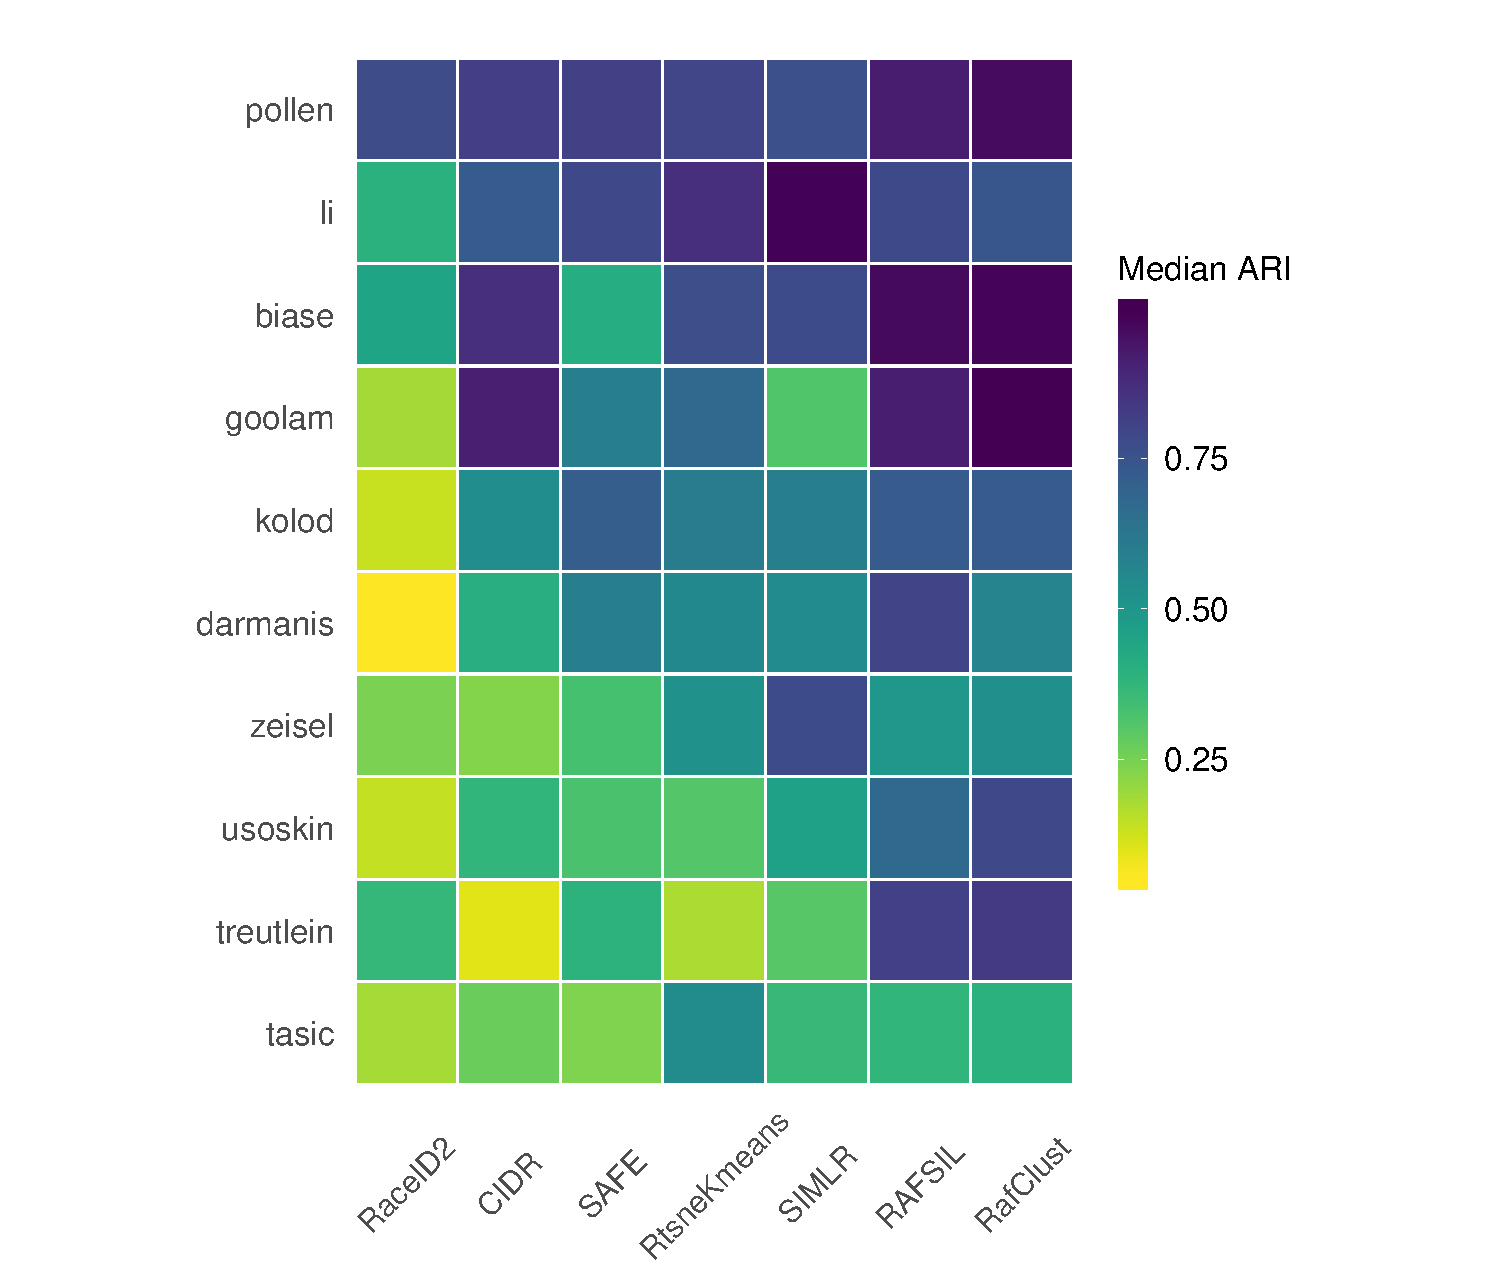
\includegraphics[width=0.9\textwidth]{Figure_ari_summary.pdf}
    \caption{
    % Median ARI across different runs on the same dataset for the methods
    不同数据集上不同方法的~ARI~中位数结果,颜色越深表示~ARI~中位数值越高。
    }
    \label{fig:rafari}
\end{figure}

在这十个数据集上,我们选择了~Goolam~和~Usoskin~两个数据集进行了数据集和聚类结果可视化。
从图~\ref{fig:rafari}~可知~SIMLR、RAFSIL~这两种方法的~ARI~仅次于方法~RafClust,
因此我们选用它们跟~RafClust~对比,在这两个数据集上对聚类结果进行了可视化, 
如图~\ref{fig:usoskin-tsne}~和~\ref{fig:goolam-tsne}~所示。
总体上来看,~SIMLR~和~RAFSIL~均比原始数据上直接进行~t-SNE~结果要好,
RafClust~表现比~SIMLR、RAFSIL~这两种方法结果要好。

\begin{figure}[!htbp]
  \centering
  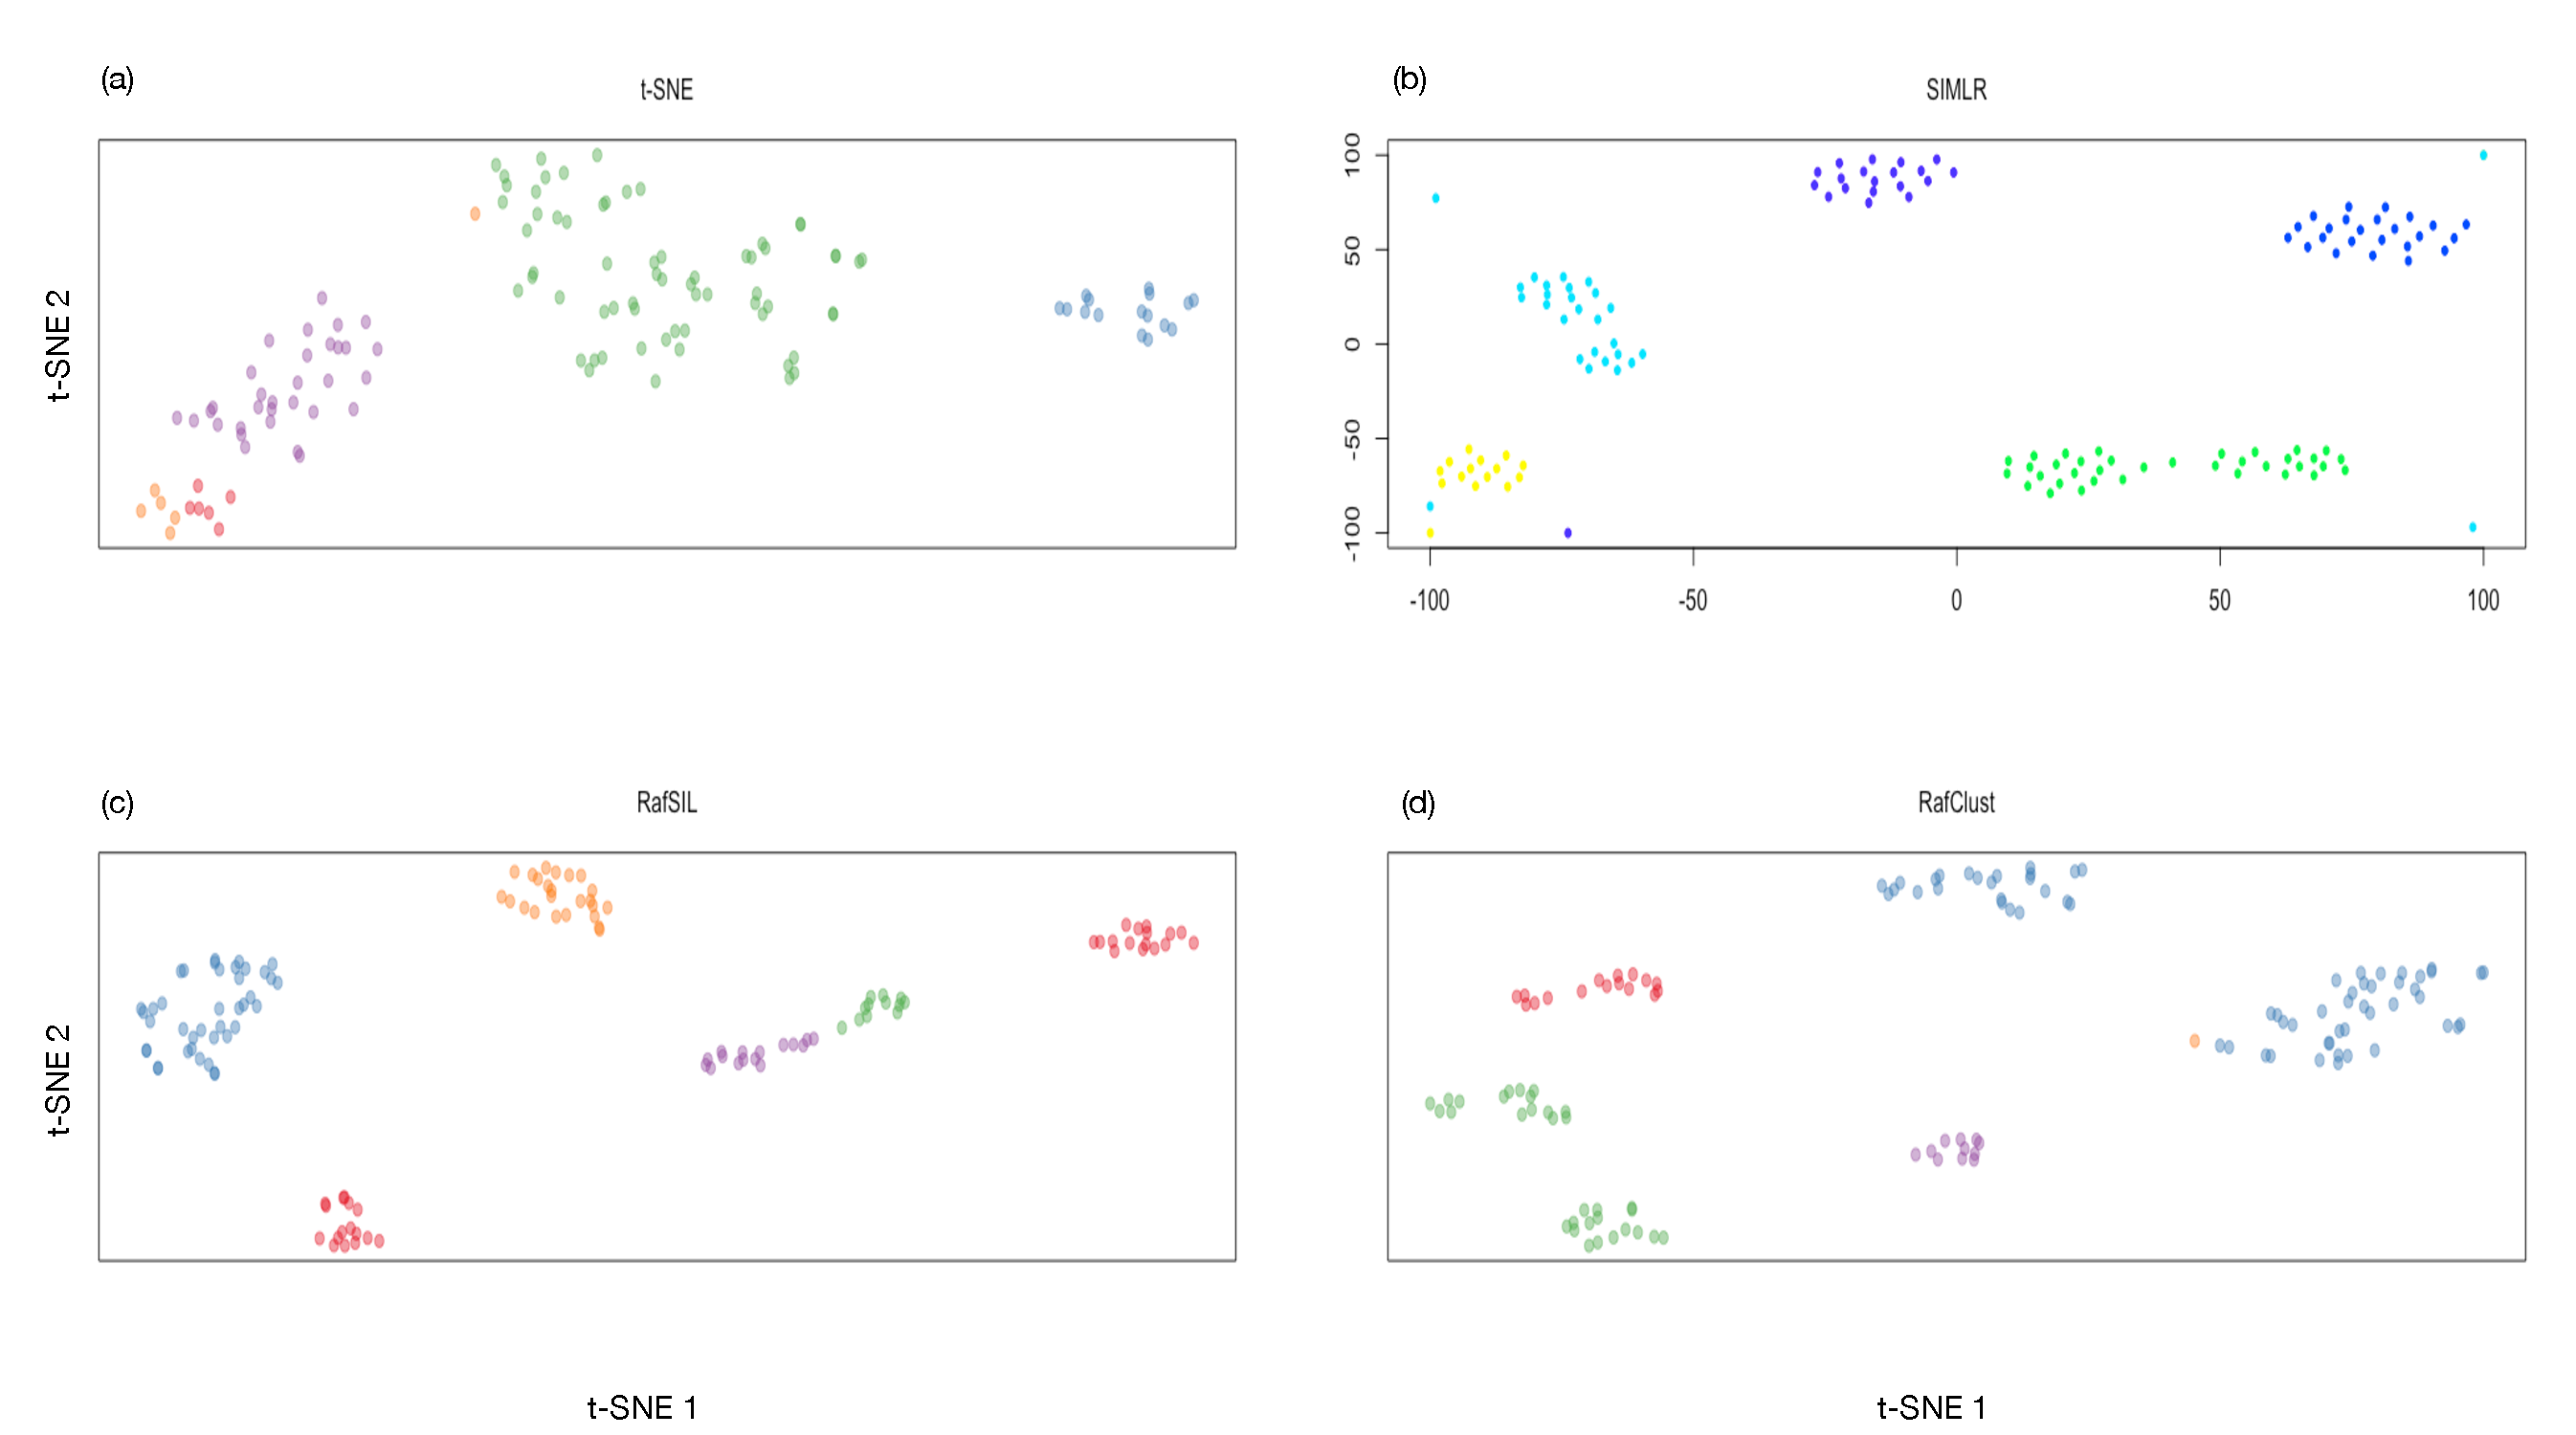
\includegraphics[width=0.9\textwidth]{goolam-tsne.pdf}
  \caption{
  Goolam~数据集上的可视化。
  (a) 原始数据集使用~t-SNE~可视化,使用了真实的细胞类别标签进行着色,参数~perplexity~设置为~20。
  (b) ~SIMLR~方法聚类结果可视化。
  (c) ~RAFSIL~方法聚类结果可视化,参数~perplexity~设置为~20。
  (d) ~RafClust~方法聚类结果可视化,对距离矩阵使用~t-SNE~进行可视化,参数~perplexity~设置为~20。
  }
  \label{fig:goolam-tsne}
\end{figure}


\begin{figure}[!htbp]
  \centering
  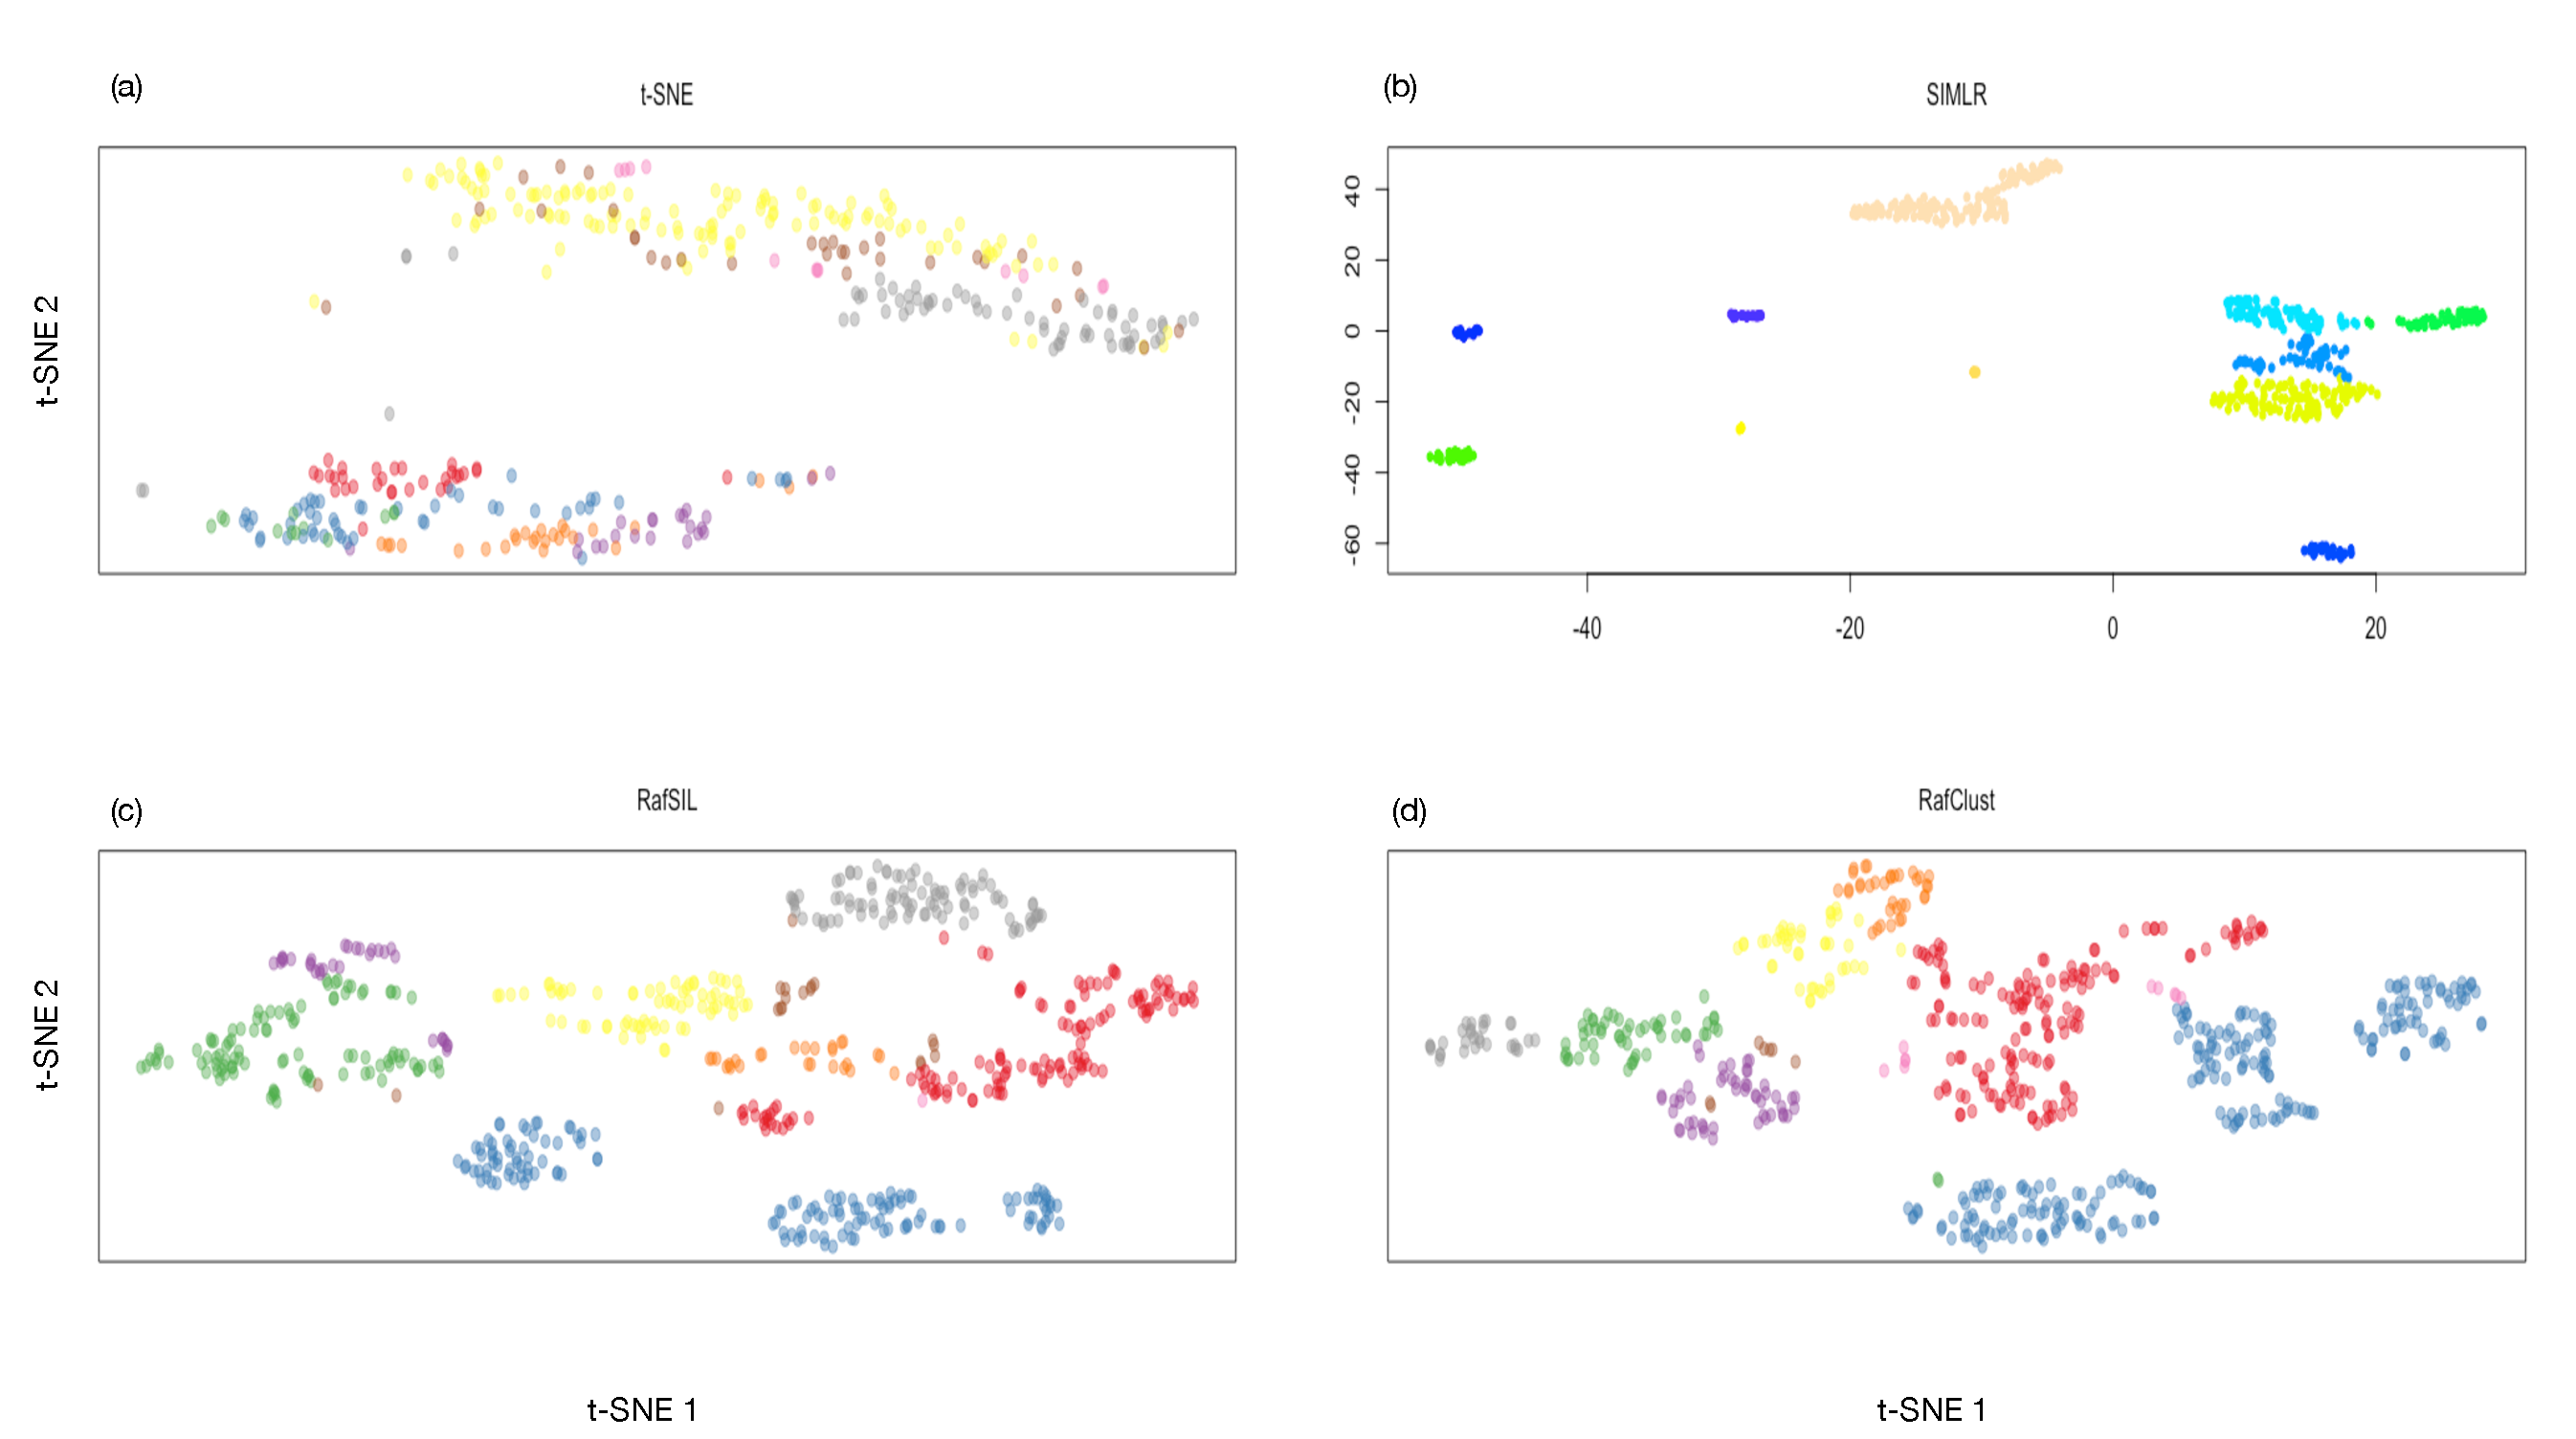
\includegraphics[width=0.9\textwidth]{usoskin-tsne.pdf}
  \caption{
  Usoskin~数据集上的可视化。
  (a) 原始数据集使用~t-SNE~可视化,使用了真实的细胞类别标签进行着色,参数~perplexity~设置为~20。
  (b) ~SIMLR~方法聚类结果可视化。
  (c) ~RAFSIL~方法聚类结果可视化,参数~perplexity~设置为~20。
  (d) ~RafClust~方法聚类结果可视化,对距离矩阵使用~t-SNE~进行可视化,参数~perplexity~设置为~20。
  }
  \label{fig:usoskin-tsne}
\end{figure}

\subsection{小结}

RafClust~是一种纯粹的无模型~(model free)~和数据驱动~(data driven)~的方法,
不需要其它的先验信息,如细胞或基因的群体结构、通路信息等。
该方法聚类的时候既可以支持外部指定细胞的类别数, 也可以让方法自己决定细胞的类别数,
还支持聚类结果的可视化和差异基因分析。
RafClust~的~R~包可在~GitHub~仓库~\url{https://github.com/chenxofhit/RafClust}~上下载和使用,
本章节相关的实验代码和相关数据集可以根据用户的要求提供。

单细胞测序从最初在转录组、基因组中的成功应用, 逐渐席卷到包括基因组、转录组、蛋白质组、表观组等各个组学。
单细胞~RNA-seq~(scRNA-seq)、单细胞~ATAC-seq~(scATAC-seq)、单细胞~Hi-C~(scHi-c)~等已成为最重要的数据类型。
这些数据主要从~mRNA~表达量、染色质的三维结构、染色质可达性等不同方面反应了细胞的信息。
细胞异质性研究中可以结合这三种异构数据进行融合,~RafClust~中构造细胞表达的特征矩阵是后续利用随机森林算法的基础,
这个步骤十分适合结合这三种异构数据直接构造细胞的特征矩阵。
后续,我们将关注融合单细胞多元组学的数据进行细胞的异质性研究。

本章中,我们提出了一种高效准确的单细胞聚类方法~RafClust。
我们使用多种相似性度量方法刻画细胞的特征,
使用随机森林回归模型来学习细胞与细胞之间的相似性矩阵,基于相似性矩阵后采用层次聚类来决定细胞的最终类别。
实验结果表明, 在十个单细胞数据集上,~RafClust~在~ARI~上表现优于其它六种方法。


